%                                                                 aa.dem
% AA vers. 8.2, LaTeX class for Astronomy & Astrophysics
% demonstration file
%                                                       (c) EDP Sciences
%-----------------------------------------------------------------------
%
%\documentclass[referee]{aa} % for a referee version
%\documentclass[onecolumn]{aa} % for a paper on 1 column  
%\documentclass[longauth]{aa} % for the long lists of affiliations 
%\documentclass[rnote]{aa} % for the research notes
%\documentclass[letter]{aa} % for the letters 
%\documentclass[bibyear]{aa} % if the references are not structured 
% according to the author-year natbib style

%
\documentclass[printer]{aa}  

%
\usepackage{graphicx}
\usepackage{caption}
\usepackage{subcaption}
%%%%%%%%%%%%%%%%%%%%%%%%%%%%%%%%%%%%%%%%
\usepackage{txfonts}
%%%%%%%%%%%%%%%%%%%%%%%%%%%%%%%%%%%%%%%%
%\usepackage[options]{hyperref}
% To add links in your PDF file, use the package "hyperref"
% with options according to your LaTeX or PDFLaTeX drivers.
\usepackage{pseudocode}
%
% Enable mutiple title row on tables.
\usepackage{multirow}
%%%%%%%%%%%
% 
% Dealing with ``too many unprocessed floats'' use it with \clearpage 
\usepackage[section] {placeins}

% For marginal notes
\usepackage{marginnote}
\usepackage{booktabs}

\begin{document} 


   \title{Physical parameter estimates of M-type stars: a machine learning perspective.}

   \author{
          L. M. Sarro \inst{1}  
          \and
          J. Ordieres-Mere \inst{2} 
          \and
          A. Bello-Garcia\inst{3} 
          \and
          A. Gonzalez-Marcos\inst{4} 
          \and
          M.B. Prendes-Gero\inst{3} 
          }

   \institute{ 
      \inst{1} Universidad Nacional de Educaci\'{o}n a Distancia, \\
               Department of Artificial Intelligence.
               \email{lsb@uned.es}
        \and 
      \inst{2}  Universidad Polit\'{e}cnica de Madrid (UPM), PMQ Research Group, \\
              Jos\'{e} Guti\'{e}rrez Abascal 2, 28006 Madrid, Spain. 
              \email{j.ordieres@upm.es}
        \and 
      \inst{3}   Universidad de Oviedo, Construction and Manufacturing Engineering Department, \\
              Campus de Viesques s/n, Gij\'{o}n, Asturias, Spain. 
              \email{\{abello,mbprendes\}@uniovi.es} 
        \and 
      \inst{4}  Universidad de la Rioja, P2ML Research Group, \\
              Luis de Ulloa 20, 26004 Logro\~{n}o, La Rioja, Spain. 
              \email{ana.gonzalez@unirioja.es}
      }

   \date{Received \today; accepted }

% \abstract{}{}{}{}{} 
% 5 {} token are mandatory
 
  \abstract
  % context heading (optional)
  % {} leave it empty if necessary  
%    {To investigate the physical nature of the `nuc\-leated instability' of
%    proto giant planets, the stability of layers
%    in static, radiative gas spheres is analysed on the basis of Baker's
%    standard one-zone model.}
%   % aims heading (mandatory)
%    {It is shown that stability
%    depends only upon the equations of state, the opacities and the local
%    thermodynamic state in the layer. Stability and instability can
%    therefore be expressed in the form of stability equations of state
%    which are universal for a given composition.}
%   % methods heading (mandatory)
%    {The stability equations of state are
%    calculated for solar composition and are displayed in the domain
%    $-14 \leq \lg \rho / \mathrm{[g\, cm^{-3}]} \leq 0 $,
%    $ 8.8 \leq \lg e / \mathrm{[erg\, g^{-1}]} \leq 17.7$. These displays
%    may be
%    used to determine the one-zone stability of layers in stellar
%    or planetary structure models by directly reading off the value of
%    the stability equations for the thermodynamic state of these layers,
%    specified
%    by state quantities as density $\rho$, temperature $T$ or
%    specific internal energy $e$.
%    Regions of instability in the $(\rho,e)$-plane are described
%    and related to the underlying microphysical processes.}
%   % results heading (mandatory)
%    {Vibrational instability is found to be a common phenomenon
%    at temperatures lower than the second He ionisation
%    zone. The $\kappa$-mechanism is widespread under `cool'
%    conditions.}
%   % conclusions heading (optional), leave it empty if necessary 
   {}

   \keywords{class M stars --
                dynamic feature selection --
                physical parameter identification --
                Temperature, gravity and metalicity Modelling --
                Learning from BT-Settl spectra library
               }

   \maketitle
%

{\bf TODO: Luis, cambiar spectral libraries por stellar atmosphere
models o synthetic spectral libraries}.
   
\section{Introduction}
\label{sec:intro}

% The importance of M stars
% The problem of estimation of stellar parameters in the M regime: bands, no continuum...
% who and what. Teff calibrations
% \cite{rajpurohit}
% \cite{amelia}

% Atlases 
%\cite{2013arXiv1306.3709B} % for lambda > 1.1 um :(
%\cite{2009ApJS..185..289R} %IRTF library of cool star

%\cite{2012ApJ...748...93R} % Metall. and Teff indicators in the K band! :(

% Summary of spectral diagnostics in the IR for M stars


\section{Methodology. \label{meth}}
The objective addressed in this Section is to develop a procedure to
identify spectral bands that yield good temperature, gravity and
metallicity diagnostics. Given the lack of a calibration set of
observed spectra with homogeneous coverage of the space of physical
parameters, we turn to synthetic libraries of spectra. Furthermore,
only temperatures and gravities can be calibrated independently of the
spectra: all metallicity estimates in the literature are based on
collections of synthetic spectra, and therefore spectral synthesis
codes are the only resource to construct regression models.

The atomic or molecular line/band parameters could in principle
indicate the spectral features that are more sensitive to changes in
the physical parameters. The suitability of spectral features as
diagnostics ofthe stellar atmospheric properties depends not only on
the individual behaviour of each line/band, but also on the relative
properties of neighbouring features in the same spectral region, that
may overlap depending on the spectral resolution. Furthermore, good
spectral diagnostics at a given signal-to-noise ratio (SNR) may show a
severely degraded predictive power in the low SNR regime. In the
following we adopt the BT-Settl library of synthetic spectra
(\cite{2013MSAIS..24..128A}) as the framework where spectral
diagnostics will be searched for. These synthetic spectra were
pre-processed in several steps as described below.

\subsection{Spectral preprocessing}

First, and in order to define good temperature diagnostics, spectra
between 2000 and 4200K in steps of 100 K were selected, with $\log(g)$
in the range between 4 and 6 dex (when g is expressed in cm/s$^{-2}$),
in steps of 0.5 dex. The metallicity of the representative spectra was
restricted to the set 0, 0.5 and -1 dex.  This yields a total set size
of 535 available spectra.

A series of preprocessing steps were then carried out in order to
match the spectral resolution and wavelength coverage and sampling of
the synthetic library to that of the collection of observed spectra
(IPAC or IRTF, see below). This required the definition of a common
wavelength range present in all available observed spectra, and the
subsequent trimming to match that range. A unique wavelength sampling
was also defined and all spectra (synthetic and observed) interpolated
to match the sampling. Finally, all spectra, both synthetic and
observed were divided by the integrated flux in order to factor out
the stellar distance.

%%%%%%%%%%%%%%%%%%%%%%%%%%%%%%%%%%%%%%%%%%%%%%%%%%%%%%%%%%%%%%%%%%%%%%%%%
%                          TO BE REMOVED
%%%%%%%%%%%%%%%%%%%%%%%%%%%%%%%%%%%%%%%%%%%%%%%%%%%%%%%%%%%%%%%%%%%%%%%%%
%In order to increase the density of examples in parameter space, we
%introduced interpolated spectra in the BT-Settl grid. Interpolation
%was obtained as a linear combination of spectra in the grid, weighted
%by the inverse square of the euclidean distance. {\bf Aqui, la
%distancia euclidea deberia calcularse en parametros normalizados,
%porque si no la temperatura domina la distancia. Fue asi?} We compared
%a set of interpolated spectra with those produced using the PHOENIX
%code (\cite{fuhrmeister2005phoenix}) to be sure that interpolation was
%a valid solution to infer new synthetic spectra. {\bf Yo aqui daría el
%RMSE de reconstruccion, mejor que la figura comp-gen-inter}

%(see Fig.~\ref{fig:comp_gen_inter}).  }

%\begin {figure}
% \begin{center}
% 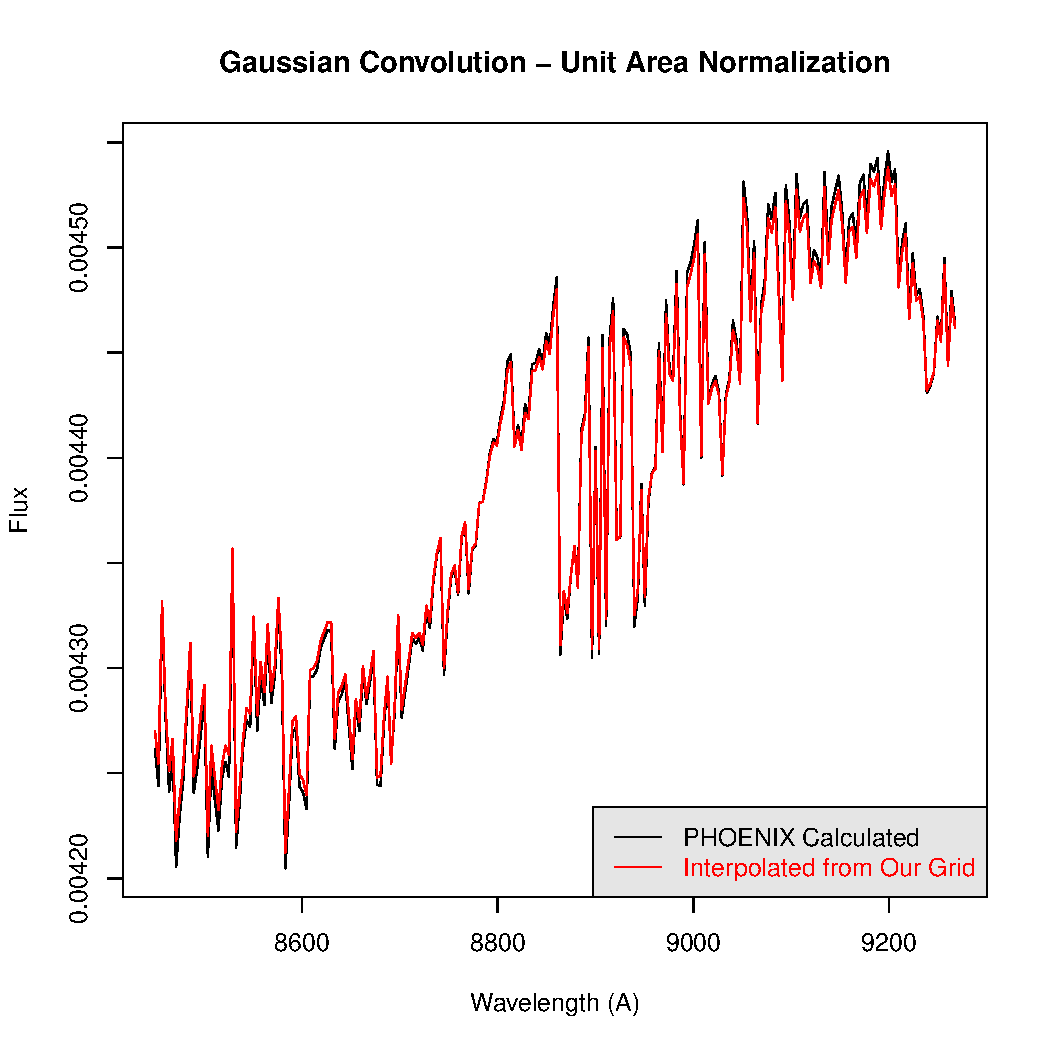
\includegraphics[width=6cm]{figs/intgrid4_gauss.pdf}
% \caption{Comparison between generated and interpollated spectrum}
% \label{fig:comp_gen_inter}
% \end{center}
%\end {figure}

%A first interpolation stage allowed us to define a finer mesh step of
%0.25 dex for both, $\log(g)$ and metallicity and 50K in temperature,
%yielding a total 1329 spectra.  Then, a second interpolation stage
%refined the grid down to 25 K in temperature and 0.125 dex in
%$\log(g)$, keeping the metallicity step at 0.25 dex and producing a
%dataset with 25912 spectra.  In spite of these, and in order to keep
%their knowledge closer to the original BT-Settl source, most of the
%analyses have been performed with the original 535 spectra
%dataset.{\bf Habría que delimitar exactamente donde se han utilizado
%535 y dónde 25912. Si la mayoria del analisis se ha realizado sobre
%535, no se si tiene sentido incluir la parte de interpolacion.}
%%%%%%%%%%%%%%%%%%%%%%%%%%%%%%%%%%%%%%%%%%%%%%%%%%%%%%%%%%%%%%%%%%%%%%%%%%

In order to avoid selecting spectral features that are good predictors
only in the unrealistic SNR=$\infty$ regime, the search for optimal
diagnostics of the atmopheric paramters of M stars was carried out for
three SNR values (10, 50 and $\infty$) by degrading the synthetic
spectra with Gaussian noise of zero mean. These values were found to
be sufficient in a wide range of experiments carried out in parallel
and described in \cite{Anaetal}.

\subsection{Feature definition and selection}
\label{subsec:FD}
As mentioned in Sect. \ref{sec:intro}, it is well known the
difficulty in defining good spectral diagnostics for M stars in the
infrared.

The work in \cite{cesetti} defined wavelength regions in the I and K
bands optimal for the diagnostic of physical parameters based on the
sensitivity exhibited by the flux emitted in these segments to changes
of the physical parameters. The sensitivity was measured in terms of
the derivative of the flux with respect to the physical parameter. The
approach adopted in this work is to select spectral features that
yield the best accuracy when used as predictive variables in a
regression model that estimates the stellar atmospheric physical
parameters ($T_{eff}$, $\log(g)$ and metallicity). The evaluation of
the accuracy of the estimates produced from a subset of features is
described further below. We consider the effective temperature as the
dominant parameter influencing changes in the stellar spectra (a
strong feature) and thus, it was estimated first, and then used as in
the regression models for the gravity and metalicity.

Here, a feature $F$ is defined as

\begin{equation}\label{eq:featureDefinition}
  F = \int_{\lambda_{1}}^{\lambda_{2}} (1-\frac{f(\lambda)}{F_{cont}} \cdot {\rm d}{\lambda})
\end{equation}

where $f(\lambda)$ denotes the normalized flux from the star at
wavelength $\lambda$, and where $F_{cont}$ is the average flux in a
spectral band between $\lambda_{cont;1}$ and $\lambda_{cont;2}$. We
explain below how we search for the band definitions that produce
physical parameter predictions with the smallest errors.

Another type of features defined as

\begin{equation}\label{eq:feature2}
  F' = \frac{ \int_{\lambda_{1}}^{\lambda_{2}}f(\lambda) \cdot {\rm d}{\lambda}}
               {\int_{\lambda_{3}}^{\lambda_{4}} f(\lambda) \cdot {\rm d}{\lambda}} 
\end{equation}

were considered, where $\lambda_1, \lambda_2, \lambda_3$, and
$\lambda_4$ delimit two spectral bands such that the ratio of the
integrated fluxes in the two bands is hoped to be a good predictor
(alone or in combination with other features) of the star atmospheric
physical parameters. The results obtained with this alternative
feature definition did not differ significantly on average from the
ones observed with the one adopted in Eq. \ref{eq:featureDefinition}, and
including them here would result in an excessively lengthy paper. In
view of the equivalent global performances, we prefered the former
because it allows direct comparison with the features proposed
by \cite{cesetti}.

We used Genetic Algorithms to solve the optimization problem described
above, that is, the problem of finding the features (band boundaries)
that minimize the prediction error of a regression estimate of the
physical parameters. We used the implementation of genetic algorithms
publicly available as the R \citep{R2013} GA  package. The concept of
using in-silico evolution for the solution of optimization problems
was introduced by \cite{holland1975adaptation}. Although its
application is now reasonably widespread \citep[see
e.g. ]{goldberg1989genetic}), they became very popular only when
sufficiently powerful computers became available. {\bf Aquí hay que
citar trabajos en astrofísica que utilicen GA y, en particular, un
artículo de Charbonneau
http://adsabs.harvard.edu/abs/1995ApJS..101..309C en 1995 que fue como
la presentación en sociedad.}

For the sake of simplicity let us define Genetic Algorithms (GAs) as
search algorithms that are based on the principle of evolution by
natural selection. The procedure works by evolving (in the sense
explained below) sets of variables (chromosomes) from an initial
random population. Evolution proceeds via cycles of differential
replication, recombination and mutation of the fittest
chromosomes. The concept of fittest is context dependent, but in our
case fitness is defined in relation with the accuracy with which a
given chromosome (set of spectral features ${F_i}$) predicts the
physical parameters.

The implementation of the GA comprises the following steps:

\begin{itemize}
\item [\textbf{Stage 1}:]{Definition of the population of potential features (chromosomes).}
\item [\textbf{Stage 2}:]{Each chromosome in the population is evaluated by its ability to
predict the physical paramters of each star in the dataset (fitness
function).}
\item [\textbf{Stage 3}:]{Chromosome selection, when a chromosome has 
 a score higher than a predefined value.}
\item [\textbf{Stage 4}:]{The population of chromosomes is replicated. 
 Chromosomes with higher fitness scores will generate more numerous
 offspring.}
\item [\textbf{Stage 5}:]{The genetic information contained in the replicated parent
chromosomes is combined through genetic crossover. Two randomly
selected parent chromosomes are used to create two new chromosomes.}
\item [\textbf{Stage 6}:]{Mutations are then introduced in the chromosome randomly. 
 These mutations produce new genes used in chromosomes.  Steps 5 and 6
 are applied over the chromosomes established at Step 4.}
\item [\textbf{Stage 7}:]{This process is repeated from Stage 2 until 
  a target accuracy is achieved or the maximum number of iterations is
  attained.}
\end{itemize}

We test features (both for the numerator and denominator of
Eq. \ref{eq:featureDefinition}) that comprise ten consecutive spectral
bins of the spectrum. These features may overlap by as much as 5
consecutive bins (which in practice implies that we define the first
feature as the spectral chunk between wavelength bins $i=1$ and
$i=10$, the second feature between bins $i=6$ and $i=15$, the third
feature between bins $i=11$ and $i=20$, etc). We do not test for
feature ratios that overlap in wavelength.


An obvious conceptual limitation of a univariate approach (considering
chromosomes that code a single predictive feature) would be the lack
of consideration that features work in the context of interconnected
pathways and, therefore, it is their behavior as a group that has to
be evaluated in terms of the predictive accuracy. Multivariate
selection methods thus seem more suitable for the analysis of the
regressors since variables are tested in combination to identify
interactions between features. In this work we define a chromosome as
a set of ten individual genes, and each gene codes a pair of
non-overlapping spectral bands, the ratio of which is used as
predictor of the physical parameters according
to (\ref{eq:featureDefinition}). 

The population size was set to 8000 individuals and the maximum number
of accepted iterations set to 4000. We produced three randomly started
populations so as to provide enough initial variety. The crossover and
mutation probabilities were set to 0.85 and 0.35 respectively. Elitism
was fixed to 0.15 {\bf No hemos mencionado elitismo; hay que
mencionarlo y definirlo antes}.

Feature fitness was defined in terms of the Akaike Information
Criterion (AIC) for linearity between the potential feature against
the physical parameter.

The most frequent and efficient features were selected as candidates
to predictive variables of the physical parameters in regression
models. We used a binary codification of the chromosomes and a
parallel implementation of the GA in a farm of fifteen computers per
physical parameter. The used architecture was the CESVIMA power7 HPC
which involve processors with 8 cores and four threads per core, running by 3,3 GHz
and with 32Gb of RAM each.


The GA procedure provides us with a large collection of chromosomes.
Although these are all potential solutions of the problem, it is not
immediately clear which one should be selected for the final
regression model.  

It is relevant to say that when genes of a chromosome induced as ratio
of two gaussian variables have extremely wide wings if any of the features 
is centered arounf zero, the fitness criteria removes it as a cadidate feature
as it is not able to explain the physical parameter. 
Therefore, the single regression model should, to some
extent, be descriptive of the population. The simpler strategy
would be to use the frequency of the chromosome in the population as
criterion for inclusion in a forward selection strategy. However we
prefered to select the features based on their highest fitness as it
enhances the value of the direct contribution to explain the physical 
parameter. 
As we have accepted that compex interaction between individual features 
are possible, it was selected a fixed number of features allowing both,
enough room for developping those complex dependency relationships but
to keep the complexity of the comming regression models under control.
Therefore, it was selected ten as the suitable number of features being considered 
per physical parameter.

Once the GA has generated a proposal set of features for predicting
each of the physical parameters, the next step consists in training
the regression model to predict them based in these features.  The GA
generates a large set of proposals that they are ordered by fitness and frequency of 
participation in the final poluation. 
Features arising less than five times were discarded as they can not be 
relevant by themselves and just arising randomly by combination with other
stronger features.

In order to assess the performance of the regression models, we
compare their predictions with i) values of the physical parameters
from the literature (when available); ii) the predictions from the
popular $minimum \chi^2$ distance to spectra in the BT-Settl library.
%;
%iii) parameter predictions based on a projection pursuit regression
%model {\bf Is this correct, Joaquín? Somewhere in your first version
%of the paper it was stated that the ICA components were fed to an SVM
%with C=10 and epsilon=0.001 for temperature, and different values for
%logg and metallicity} trained with projections of the BT-Settl spectra
%onto the set of vectors resulting from an Independent Component
%Analysis (ICA); and finally, iv) predictions from a regression model
%trained with the features proposed by \cite{cesetti} (only for the
%IRTF spectra) {\bf Joaquín, aquí necesitamos explicar qué tipo de
%modelo entrenamos con las features de cesetti.}.
In the case of features proposed by \cite{cesetti}, such ranges were
directly provided by their paper and the GA based selection of features 
was, therefore, not needed.

It is worthy to said that because of the impact on the emission spectrum 
for all the pohysical parameters are the same, several strategies were 
implemented to verify to what end using hierarchical knowledge becomes
helpful to the modelling procedure. Therefore, extensive set of trials 
have been conducted to derive gravity and metallicity features with and
without temperature knowledge. Models were trained to determine the impact of
such temperature hierarchical contribution and it was found that, 
no matter of the model considered, the features determined plus the 
estimated star temperature outperform the same model without the 
temperature knowledge by about 20\% in case of gravity models and 12\%
in case of metallicity models.
Based on those results, GA features for gravity and netallicity were 
reinforced with the estimated star temperature as an additional feature.


\subsection{Models considered.}
\label {ssub:models}
For the models to be built, the same strategy was used for all the
three physical parameters $(T_{eff}, log(g), met)$ and it was to use
regression techniques over the selected set of features.  
As a classical regression problem several modelling techniques, with
specific selection of adequate parameters per method when required,
were considered: 

\begin{itemize}
 \item {Bagging with Multiadaptative Spline Regression Models \emph{(MARS)}.}
 \item {Random Forest Regression Models \emph{(RF)}.} 
 \item {K Nearest Neighbours \emph{(KNN)}.}
 \item {Generalized Boosted Regression Models \emph{(GBM)}.}
 \item {Support Vector Regression with Gaussian Kernel \emph{(SVR)}.}
 \item {MLP Neural Networks \emph{(NNET)}.}
 \item {Kernel Partial Least Squares Regression \emph{(KPLS)}.}
 \item {Rule Regression Models \emph{(RR)}.} 
 \end{itemize}


Including here a sufficient description of each and every regression
model that we trained would render the manuscript excessively
lengthy but interested readers can find additional information in 
\cite{baraud2002model,geman1992neural,elith2008working,meyer2003support,svetnik2003random}.
Suffice it to say that each one of them can be thought of as
a parametric model that predicts one physical parameter from an input
vector. The input vector can be the full normalised spectrum, the ICA
lower-dimensional representation of the full spectrum, or the spectral
features selected by \cite{cesetti} or by the GA. The model parameters
are infered (using algorithms that differ from one regression model to
the other) from a set of examples. This set of examples (spectra of
stars for which we know the physical parameters) is called the
training set, and the process by which the model parameters are
determined from the training set, is called training of the model. In
the next paragraph we give minimal details of each regression model
trained, and references for the interested reader.

As every type of model has its own set of tunable parameters as well as
its own training procedure, the authors have selected a common wrapper 
named caret  (short for C\_lassification A\_nd RE\_gression T\_raining) \cite{caret}.
This wrapper enables a common interface as well as the use of the same 
set of samples for the adopted five-folder cross-validation training
technique used. The adopted strategy for selection of parameters was 
to search throughout the grid of values.
Therefore, generally speaking the adopted procedure for learning models 
is presented in Algorithm \ref{caretp}.

\begin{pseudocode}[shadowbox]{Model Learning}{DataSet,ParRanges}
\label{caretp}
 \mathcal{S}_{ModelParameters} \GETS ParRanges \\
 \mathcal{S}_{DataFolders} \GETS Preprocess(DataSet) \\ 
 \FOREACH x \in \mathcal{S}_{ModelParameters} \DO
  \BEGIN
    \FOREACH z \in \mathcal{S}_{DataFolders} \DO
      \BEGIN
	HDS(z) \GETS \mbox{Hold-out specific samples} \\
	Model(z) \GETS Fits(\mathcal{S}_{DataFolders} \setminus HDS(z) ) \\
	Perf(z) \GETS Predicts(Model(z),HDS(z)) \\
      \END \\
    Perf(x) \GETS Average(Perf(z)) \quad \forall z \in \mathcal{S}_{DataFolders} \\
  \END \\
  
  OPS \GETS argmax(Perf(y)) \quad \forall y \in \mathcal{S}_{Modelparameters} \\
  Model \GETS Fits(DataSet, POS) \\
\end{pseudocode}


As mentioned above, the training set was constructed from the BT Settl
library of stellar spectra. The interested reader may find different
approaches in the literature to the problem of finding an optimal set
of training examples. \cite{hoggCannon} for example prefer to use real
observed spectra rather than synthetic libraries to create a
generative model in which the individual spectral fluxes are modelled
as second degree polynomials with the physical parameters as
arguments. The real observed spectra have physical parameters taken
from the literature, which in turn are almost always inferred using
synthetic spectral libraries. In our opinion, this approach does not
solve the dependence of the predicted parameters on the necessarily
imperfect synthetic libraries, but has the advantage that the relative
frequencies of examples in the training set represents better the
biases naturally encountered in surveys than the uniform sampling of
parameter space found in synthetic libraries. Recently, \cite{heiter}
have started a program to compile a set of stars with accurate
physical parameter determinations infered independently of
spectroscopic measurements and atmospheric models (as much as
possible). Unfortunately, this ambitious program only contains 34
stars of spectral types F, G, and K. In the M regime we find similar
approaches in \cite{dummy}, \cite{dummy}, and \cite{dummy}, where the
atmospheric parameters are derived using interferometric measurements
of stellar radii. Again, this only amounts to a very small number of
examples and a very sparse sampling of the parameters space.

We believe that all efforts to compile training sets of stars with
accurate, homogeneous, and reliable physical parameters derived
independently of spectroscopic measurements are valuable not only
because they allow for the improvement of the stellar atmospheric
models but also because they help increase the reliability of the
regression models by making them independent of these same atmospheric
models. But until these training sets with sufficient and homogeneous
sampling of the parameter space are available, we turn to the use of
synthetic libraries. 




\section{Physical parameters of the IRTF collection of spectra.}
%\input{irtf}
\subsection{Spectral bands}
% Rework the sentence  JOM
\textbf{
The GAs were applied to the selection of features for the
prediction of effective temperature from both, noiseless and noisy spectra.
For the IRTF wavelength range and resolution, results in the features have been included
in Table~\ref{tab:irtf-teff-noisy}. 
}
% End of update
Features are ordered by the
fitness value (according to the AIC criterion, as explained in Eq.~\ref{eq:AIC}) and 
we only consider features that are present in at least 5 sets.

% When noise is added to the BT-Settl spectra, we obtain the features
% included in Table \ref{tab:irtf-teff-noisy}.

Table % \ref{tab:irtf-teff-noiseless} and 
\ref{tab:irtf-teff-noisy}
show a very wide variety of features with very few repetitions. Only
spectral features 4, 5, 6, and 9 in the SNR=50 experiment are found
too in the SNR=$\infty$ and SNR=10 feature sets (albeit with different
continuum definitions). This reinforces the impression that the
information useful for the estimation of the effective temperatures is
spread over the entire IRTF spectrum.
%% Removing Table A3 => JOM
%\textbf{
%As a reference, it is used the Table~3 defined in \cite{cesetti}, which
%%~\ref{tab:irtf-cesetti} 
%lists the features found using sensitivity maps.
%}
% End of changes

\begin{figure*}
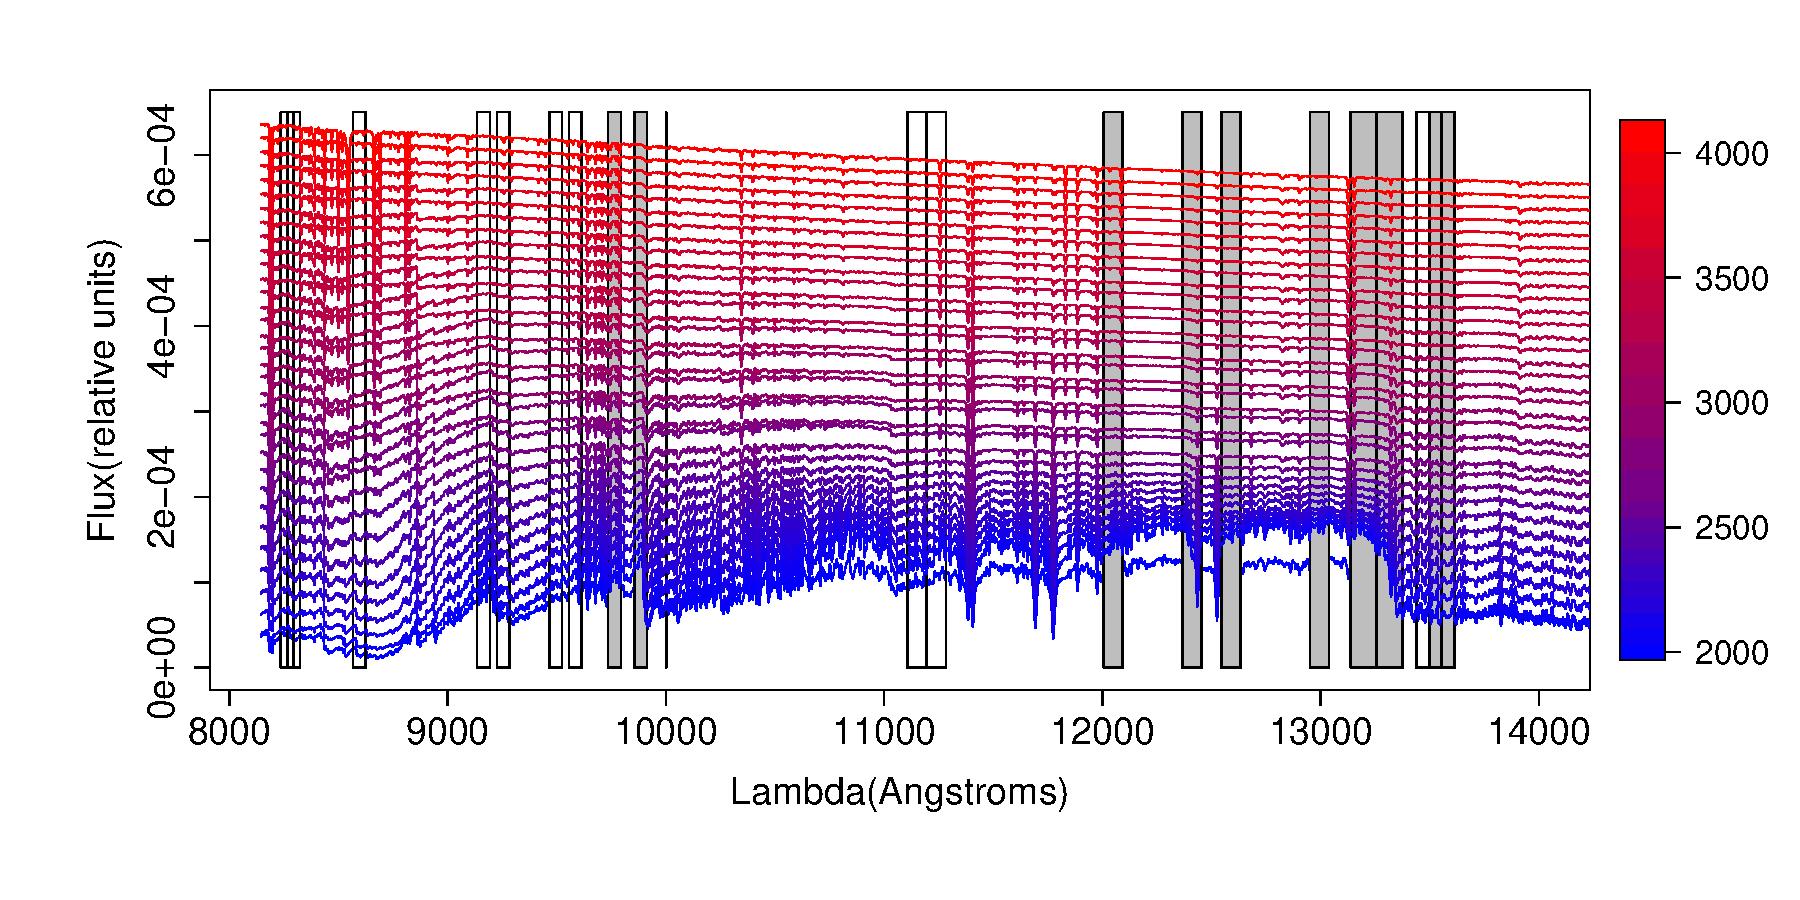
\includegraphics[width=\textwidth]{figs/BT-spectraAtIRTF-Inf-teff2}
 \caption{Features selected by the GA for predicting $T_{eff}$ using
    noiseless BT\_Settl synthetic spectra in the IRTF wavelength range
    and resolution. The BT\ Settl spectra are plot in a colour scale
    that ranges from blue (2000 K) to red (4100 K). The empty boxes
    correspond to the selected features and the grey boxes to the
    continuum bands.}  \label{fig:IRTF-teff}
\end{figure*}

For gravity estimation (on a logarithmic scale), the GA search
procedure produces the features presented in
Table % \ref{tab:irtf-logg-noiseless} and 
\ref{tab:irtf-logg-noisy} for
the noiseless signal and signal-to-noise ratios of 10 and 50,
respectively. In a similar way, the best features found 
by the GA for metallicity estimation are listed in % Table~\ref{tab:irtf-met-noiseless} for the noiseless BT-Settl
% spectra, and in 
Table~\ref{tab:irtf-met-noisy} for signal-to-noise
ratios equal to $ \infty, 10 $ and $ 50 $.

{\bf Tables~\ref{tab:irtf-teff-noisy} to \ref{tab:irtf-met-noisy}
include the band definitions for the three physical parameters and
Fig. \ref{fig:IRTF-teff} shows a graphical representation of the bands
selected for the determination of the effective temperature
superimposed on a set of noiseless BT Settl spectra.}


\subsection{Regression models}

In the following, we will summarise the results obtained for the IRTF
data set. We deal with the different physical paramenters in separate
Sections. We start by reporting the cross validation Root Mean/Median
Square Errors (RMSE/RMDSE) for the five-fold cross-validation
strategy, and subsequently discuss the accuracy of the predictions
with respect to literature values where available.

\subsection{Effective temperature models}

%%%%%%%%%%%%%%%%%%%%%%%%
%%%% Cross Validation
%%%%%%%%%%%%%%%%%%%%%%%%

Table \ref{tab:model_TSD} summarises the RMSE/RMDSE for the complete
set of models: the minimum $\chi^2$ estimate based on the full
spectrum ($\chi^2$), the projection pursuit regression based on the
ICA components (PPR-ICA) and models trained on the spectral features
proposed by the GA (GA-RF, GA-GBM, GA-SVR, GA-NNET, GA-MARS,
GA-KPLS). For each model, we report the RMSE/RMDSE obtained for
several noise levels of the training sets.  SNR=$\infty$ corresponds
to noiseless spectra. {\bf In the GA- cases, the model is trained with
  the spectral features found by the Genetic Algorithms when applied
  to BT-Settl spectra of the corresponding SNR.}

\newcommand{\ra}[1]{\renewcommand{\arraystretch}{#1}}
\begin{table*}\centering
\ra{1.3}
\begin{tabular}{@{}lrrcrrcrr@{}}\toprule
& \multicolumn{2}{c}{$SNR = 10$} & \phantom{ab}& \multicolumn{2}{c}{$SNR = 50$} &
\phantom{ab} & \multicolumn{2}{c}{$SNR = \infty$}\\
\cmidrule{2-3} \cmidrule{5-6} \cmidrule{8-9}
$Regression Models$ & $RMSE$ & $RMDSE$ && $RMSE$ & $RMDSE$ && $RMSE$ & $RMDSE$ \\ \midrule
$\chi^2$      & 232      & \bf{100.00}&& 235      & 120    && 232      & \bf{100} \\
 PPR-ICA      & 242      & 128        && 242      &  99    && 280      & 162 \\
 GA-RF        & 308      & 183        && 248      & 136    && \bf{167} & 135 \\
 GA-GBM       & 287      & 160        && 248      & 149    && 233      & 113 \\
 GA-SVR       & \bf{221} & 122        && 281      & 151    && 299      & 160 \\
 GA-NNET      & 283      & 192        && 264      & 114    && 326      & 212 \\
 GA-KNN       & 238      & 120        && \bf{232} & 137    && 219      & \bf{100}  \\
 GA-MARS      & 253      & 113        && 254      & \bf{95}&& 226      & 133 \\
 GA-KPLS      & 275      & 120        && 300      & 119    && 387      & 218 \\
\bottomrule
\end{tabular}
\caption {Cross-validation RMSE and RMDSE for the various regression
  models that predict $T_{eff}$ (K).}
\label{tab:model_TSD} 
% \end{center}
\end{table*}

Table \ref{tab:model_TSD} shows that the performance of classifiers
based on the full spectrum (or in a compressed version in the form of
ICA components) and the best classifier based on features derived from
limited spectral bands is equivalent. The difference between the
performances of the best classifier ($GA-KNN$; best on average over
SNR), the minimum $\chi^2$ classifier, and the $PPR-ICA$ classifiers
are not statistically significant. We interpret these small
differences as an indication that there is as much information spread
over the entire spectrum shape as can be distilled from a few spectral
bands. The bartlett test shows that the variances are homogeneous with
a Bartlett\textquoteright s K-squared of 8.5 with 2 degrees of freedom
and a p-value of0.01426. The Flinger-Killen test shows that
homokedascity is verified at the p=0.005886 level. Finally, the
F-ANOVA test clearly shows that there is no significant difference
between models. Thus, we conclude that the quality of features from
the two approaches are equivalent in predictive performance.  In any
case, it is evident that the RMSE is significantly above the grid
spacing in temperature.


%%%%%%%%%%%%%%%%%%%%%%%%%%%%%%%%%%%%%%%%%%%%%%%%
% Comparison with Cesetti temperatures in Table 3
%%%%%%%%%%%%%%%%%%%%%%%%%%%%%%%%%%%%%%%%%%%%%%%%

The comparison with the effective temperatures compiled by
\cite{cesetti} shows some differences across models. {\bf We have
  literature values for 57 M stars in Table 3 of \cite{cesetti}. Why
  only 57? We should have more. In Table 3 there are more than 60. Why
  is the difference? Is it because I removed some? How many?} In
general, all classifiers tend to predict lower effective temperatures
than those in the literature except in the noiseless scenario.

\begin{table*}\centering
\ra{1.3}
\begin{tabular}{@{}lrrr@{}}\toprule
& {$SNR = 10$} & {$SNR = 50$} & {$SNR = \infty$}\\ \midrule
$\chi^2 $            &  -77 &  -87  & -85 \\
$ICA+ppr$            & -104 & -55   & -130 \\
$Rule Regression$    & -102 &  -39  & 170 \\
GA-RF                & -173 & -127  &  -5 \\
GA-GBM               & -141 & -109  &  32 \\
GA-SVR               &  -58  &  -3  &  92 \\
GA-NNET              & -147 &  -36  &  39 \\
GA-KNN               &  -76  &-110  & -67 \\
GA-MARS              &  -57  & -88  &  98 \\
GA-KPLS              & -120 &   -4  & 214 \\
\bottomrule
\end{tabular}
\caption {Bias in the $T_{eff}$ (K) estimation computed with respect
  to the reference values from \cite{cesetti}.}
\label{tab:model_Tbias} 
% \end{center}
\end{table*}

It is remarkable that almost all other SNR=10 models show a tendency
to underestimate $T_{\rm eff}$ that is mitigated as we apply models of
increasing SNR. The models trained with noiseless spectra tend to
overestimate $T_{\rm eff}$, suggesting that the optimal SNR is between
SNR=50 and $\infty$. The minimum-$\chi^2$ approach and the GA-KNN
model systematically underestimate $T_{\rm eff}$ for all SNR
regimes. This concomitance is not surprising since minimum $\chi^2$ is
a single nearest neighbour method applied in the space of the entire
spectrum as opposed to the space selected features.

In general, models tend to produce better behaved solutions (with
smaller biases and less scatter) for SNR=50. We interpret this value
as representative of the SNR of the majority of spectra in the IRTF
collection. We have found in previous studies that, at least for input
spaces constructed from ICA compressions of the spectra, it is not
necessary to adapt the training set SNR to match exactly that of the
prediction set. On the contrary, we find that two regimes are
sufficient to obtain acceptable results. The two regimes are separated
at SNR=10. The model trained with SNR=50 spectra gives close to
optimal results for spectra with SNRs above 10, while below that limit
the same situation holds for the model trained with SNR=10
spectra. {\bf Cite paper by Ana.}

We then compare the predicted effective temperatures with the spectral
types listed in the IRTF spectral library. We attempted a direct
comparison with the literature values gathered in \cite{cesetti} but
it only returns 57 estimates of effective temperature for M stars. We
converted the spectral types into effective temperatures using the
calibration of \cite{2009ApJ...702..154S}.

Forecast quality of models was tested by the error against the
temperature estimated based on the Spectral Subtype for each of the
IRTF available spectra (see \ref{ssub:TLSB}).  Both Root Mean Squared
Error (RMSE) and Mean Absolute Error (MAE) where calculated and they
are presented in table~\ref{tab:model_Tvar}.

From this comparison several things arise:
\begin{itemize}
 \item {The behavior of $\chi^2$ distance is quite stable against SNR 
	in the original dataset (BT\_Settl) with a slightly better global 
	performace in fovour of SNR=50.}
 \item {Models trained with different SNR=$\infty$ have similar performance but heavy 
	differences appear when SNR features are considered.}
 \item {When synchronous behavior is observed FT00, FT11, FT55, the better SNR is 10.}
 \item {Best set of features to be used for forecast are those from SNR=$\infty$ (FT0b).}
 \item {As a conclusion the better performance was produced by FT01, followed by the FT51.}
\end{itemize}

In Figures~\ref{fig:comp01}~\ref{fig:comp02} the relationship between
Temperature estimated from the GA technique proposed features and
modeled with different techniques and the $chi^2$ with SNR=50 against
the estimations provided by \cite{cesetti} can be seen.

\begin {figure}
 \centering
 \begin{subfigure}{.85\textwidth}
  \centering
  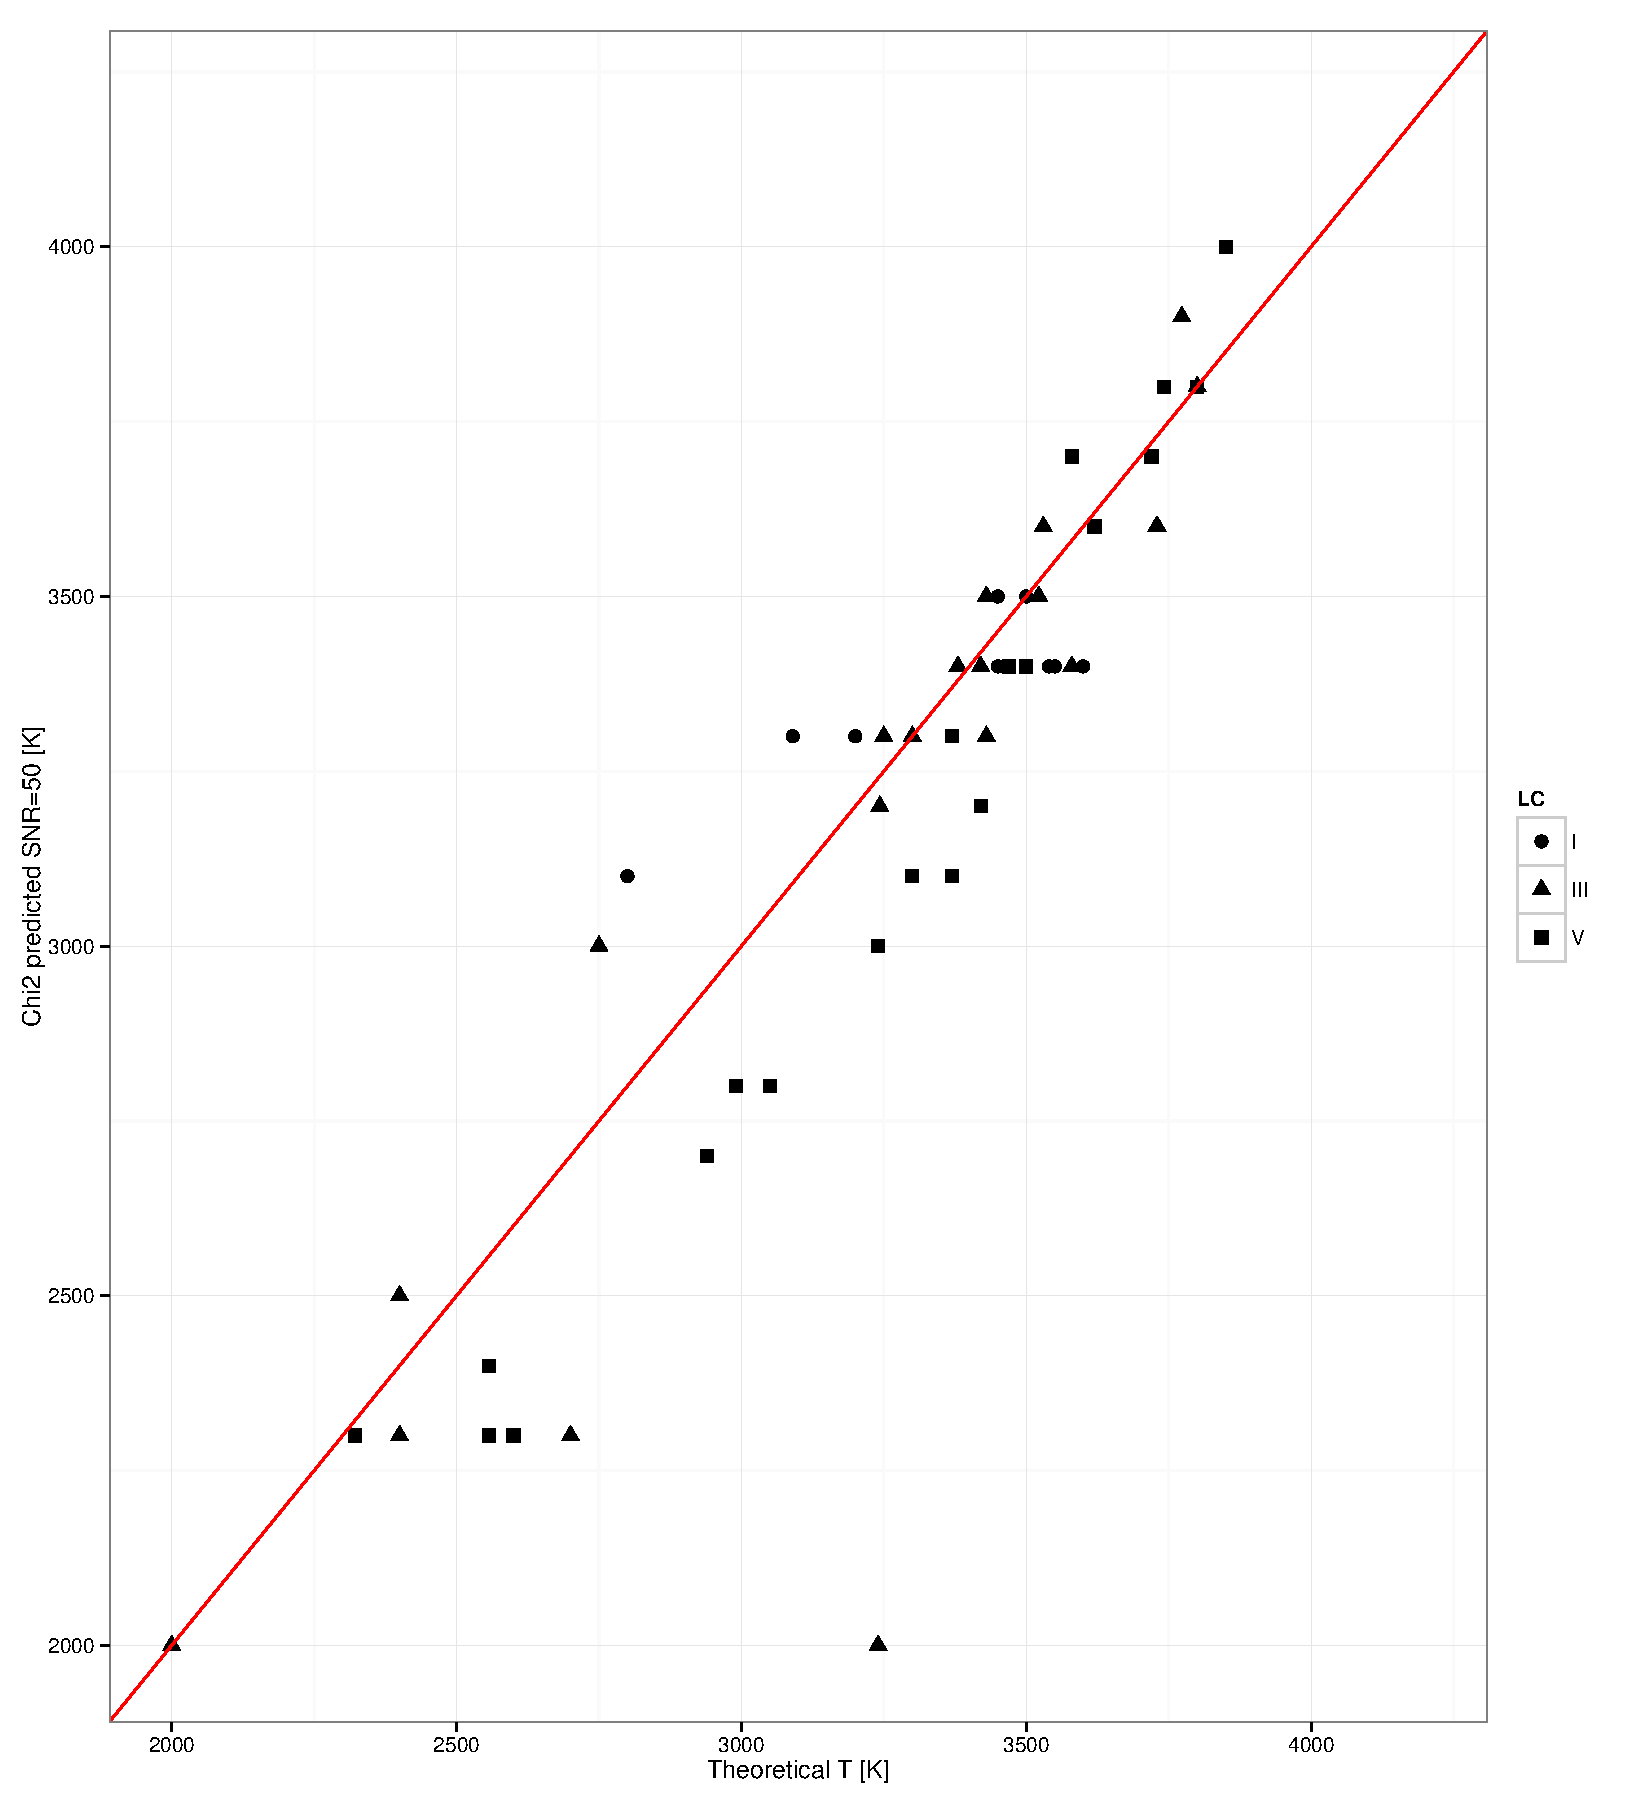
\includegraphics[width=11cm]{figs/irtf_T_chi250_Cesetti.pdf}
  \caption{Comparison between Temperature estimations from Cesetti 
  in x axis and the closest BT\_Settl spectra by $\chi^2$ at SNR=$50$ on y-axis}
 \label{fig:chi2_50_spt}
 \end{subfigure}
  \begin{subfigure}{.85\textwidth}
  \centering
  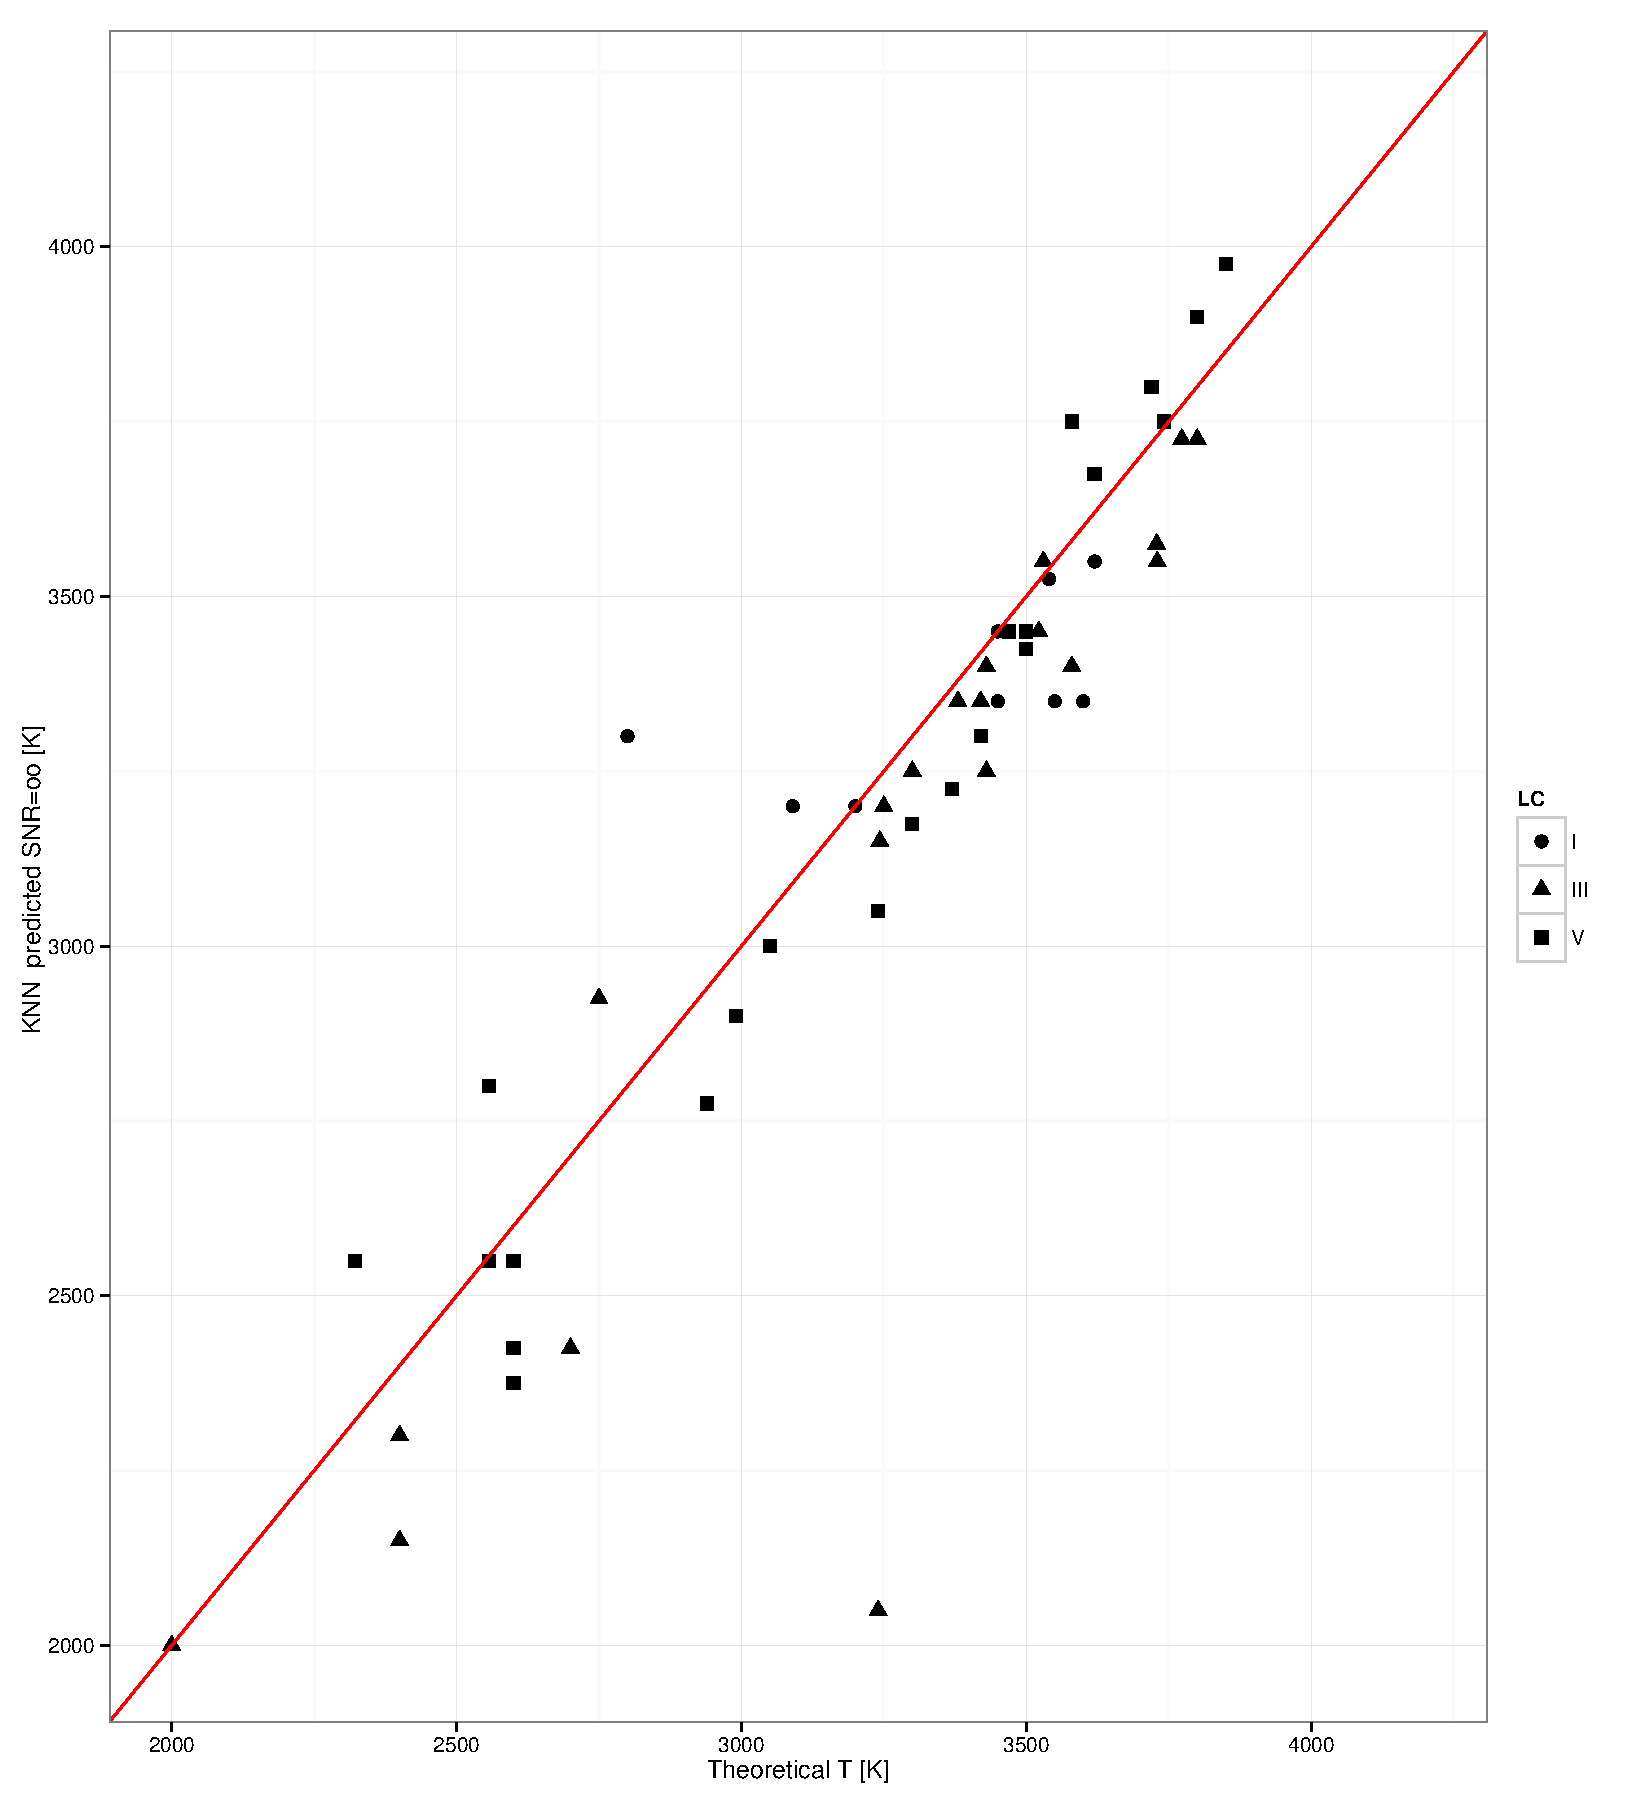
\includegraphics[width=11cm]{figs/irtf_T_knnoo_Cesetti.pdf}
  \caption{Comparison between Temperature estimations from Cesetti 
 in x axis and the KNN model for GA based features 
 at SNR=$\infty$ on y-axis}
 \label{fig:ga_too50ga_spt}
 \end{subfigure}
 \label {fig:comp01}
 \caption{Performance comparison between the $\chi^2$ based selection 
          and the band oriented features}
\end {figure}
 
 
\begin {figure}
 \centering 
 \begin{subfigure}{.85\textwidth}
  \centering
  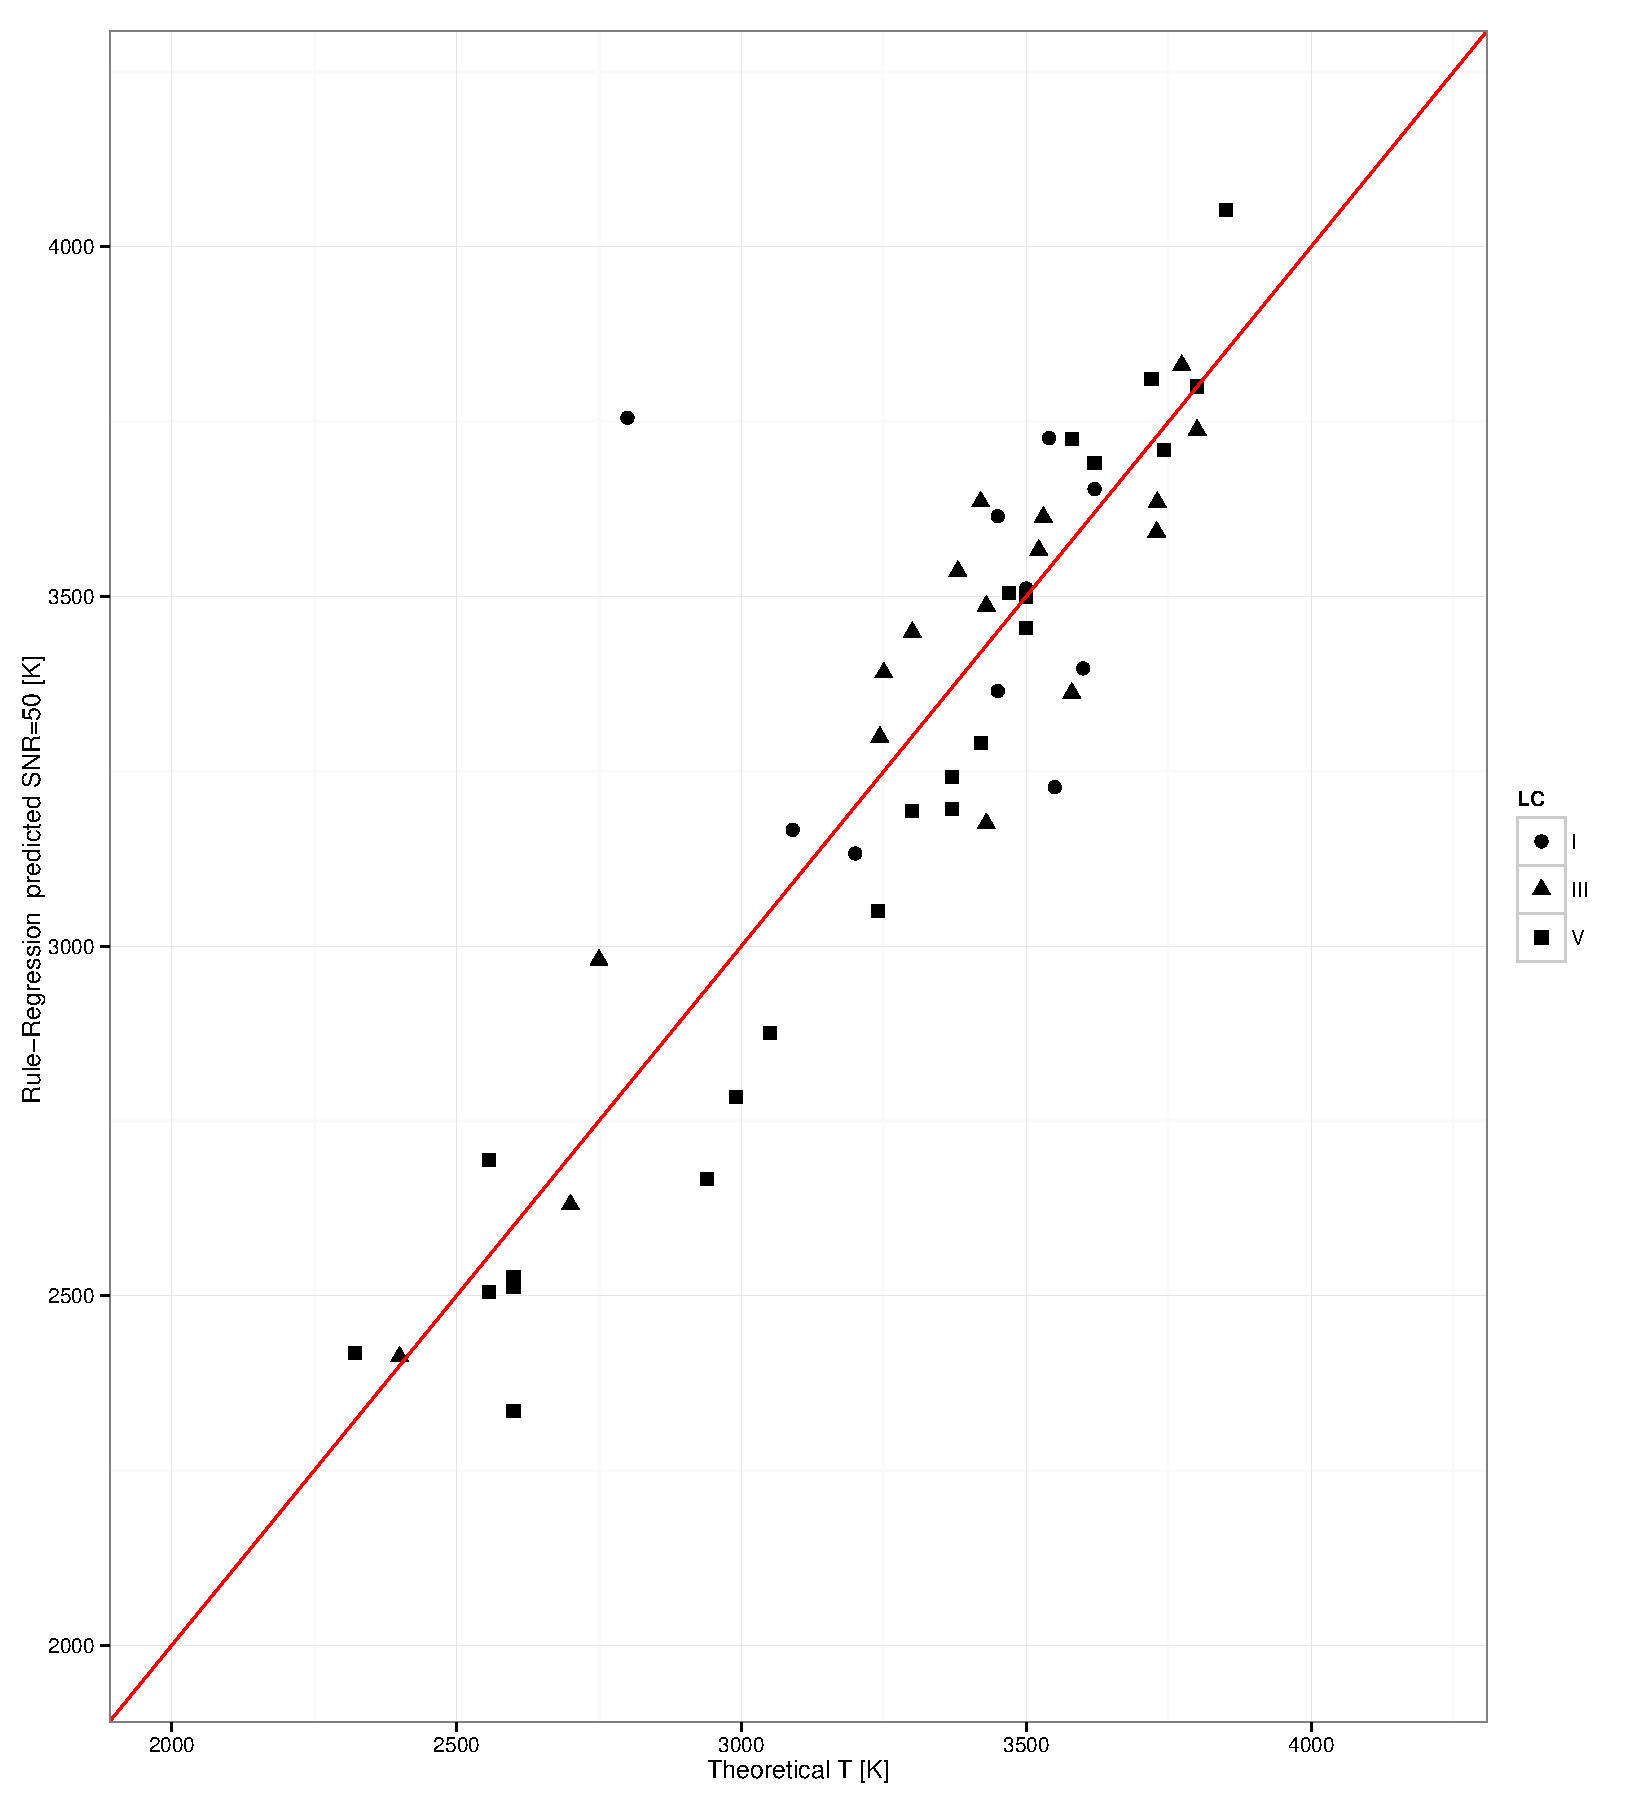
\includegraphics[width=11cm]{figs/irtf_T_rregoo_Cesetti.pdf}
  \caption{Comparison between Temperature estimations from Cesetti 
 in x axis and the Rule Regression model for GA based features 
 at SNR=$\infty$ on y-axis}
 \label{fig:ga_rr00ga_spt}
 \end{subfigure}
\begin{subfigure}{.85\textwidth}
  \centering
  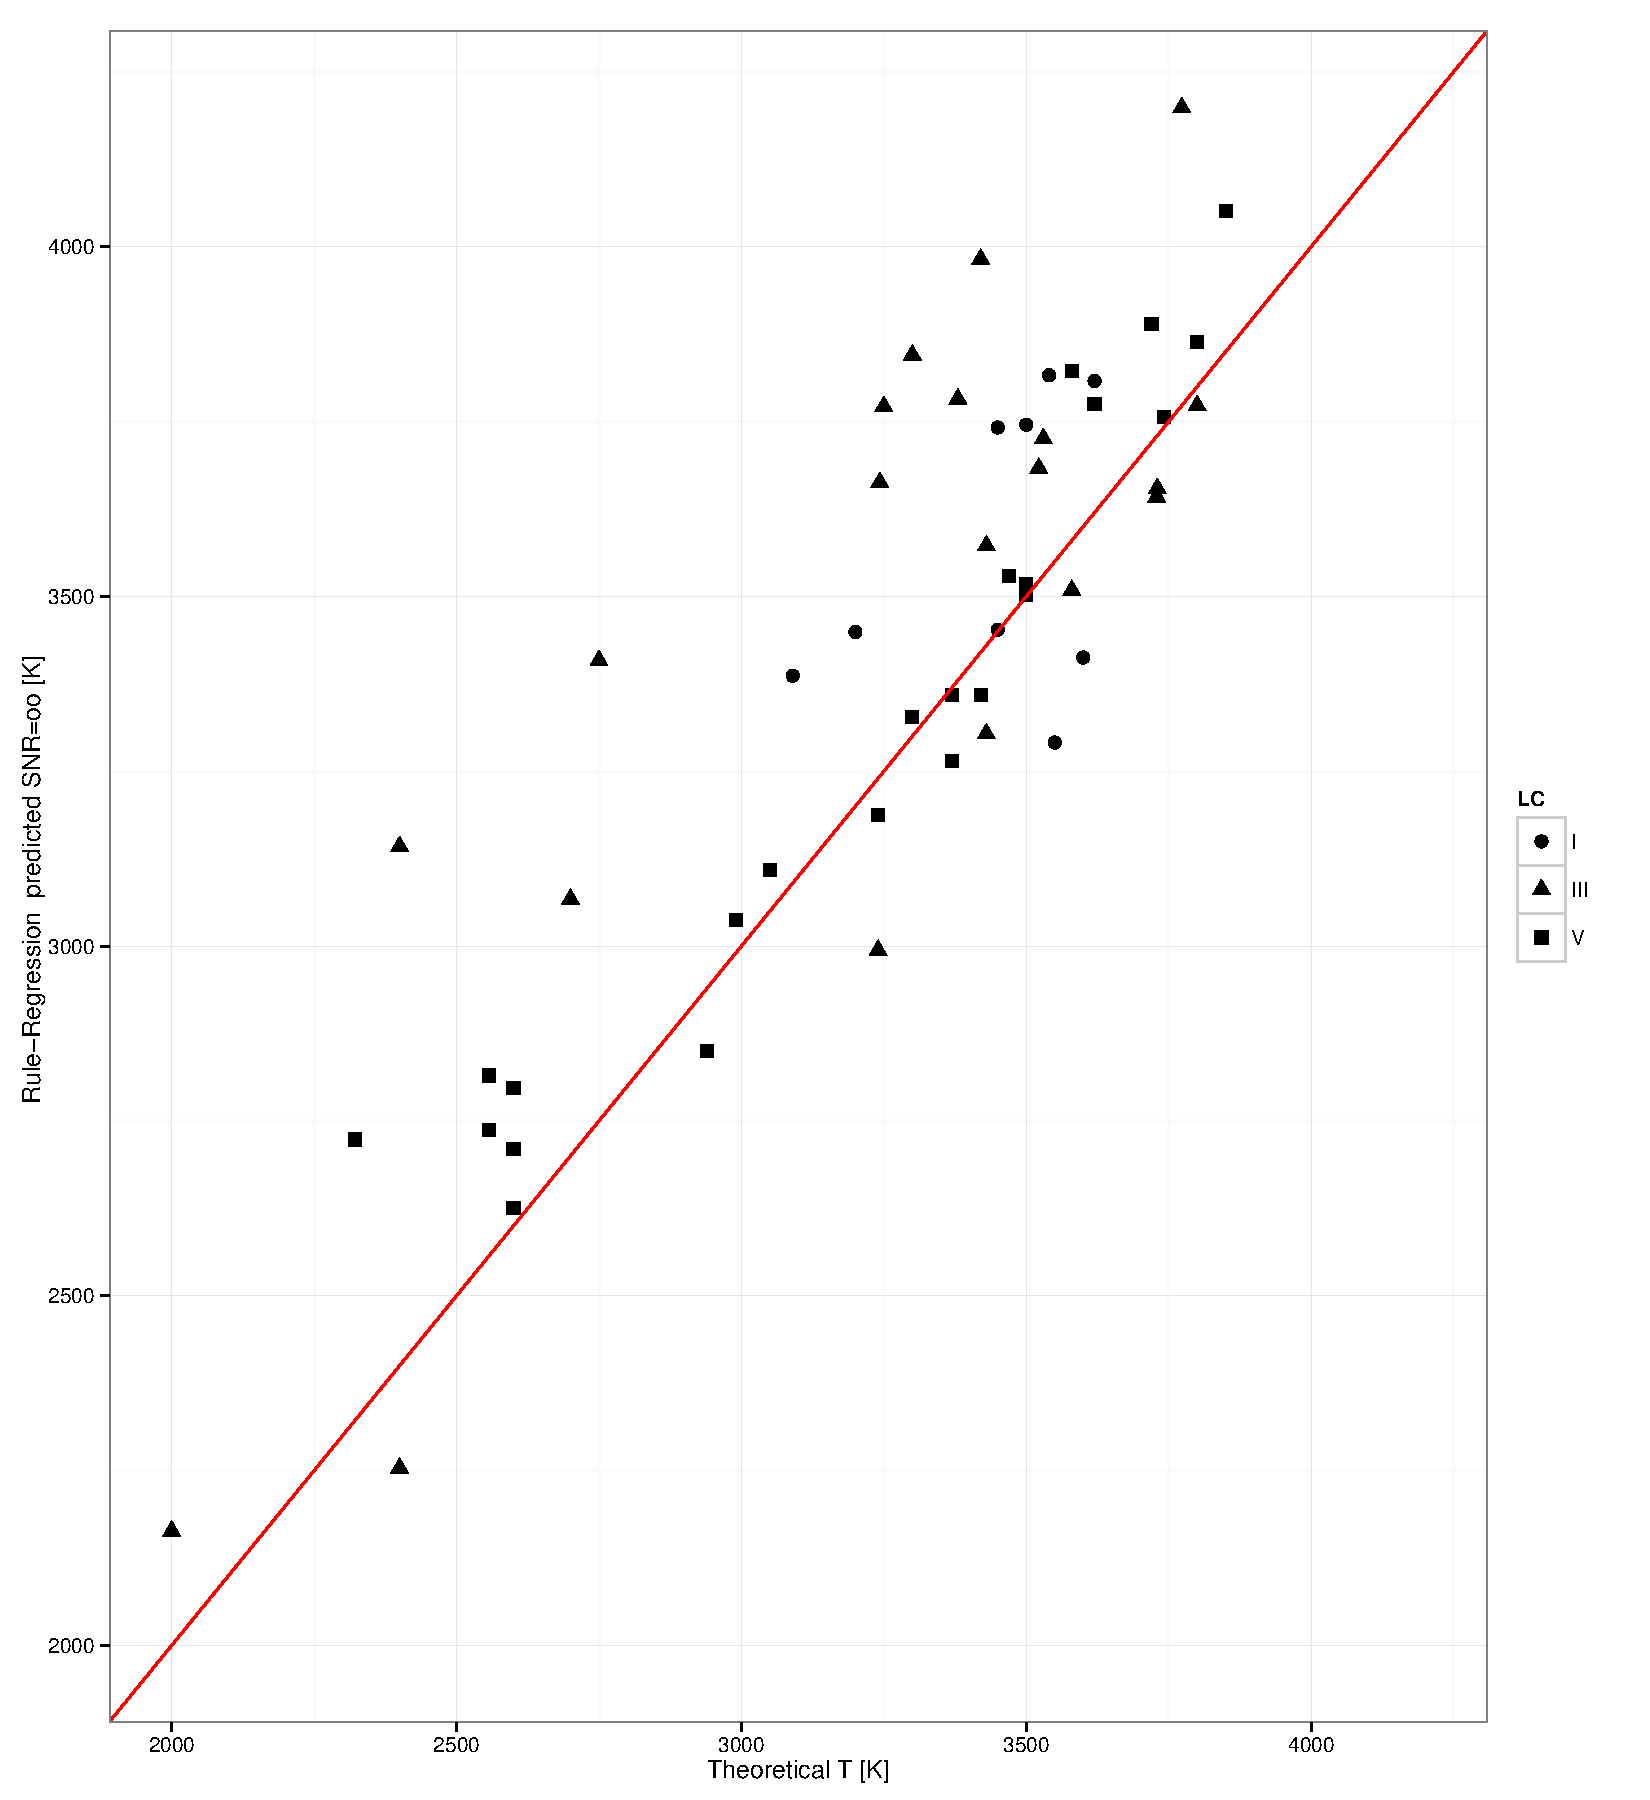
\includegraphics[width=11cm]{figs/irtf_T_rreg50_Cesetti.pdf}
  \caption{Comparison between Temperature estimations from Cesetti 
 in x axis and the Rule Regression model for GA based features 
 at SNR=$50$ on y-axis}
 \label{fig:ga_rr50ga_spt}
 \end{subfigure} 
 \label {fig:comp02}
 \caption{Performance comparison between two Rule regression based models with different SNR}
\end {figure}

%%%%%%%%%%%%%%%%%%%%%%%%%%%%%%%%%%%%%%%%%%%%%%%%%%%%%%%%%%%%%%
% TBD: Comparison with temperatures estimated with Cesetti features
%%%%%%%%%%%%%%%%%%%%%%%%%%%%%%%%%%%%%%%%%%%%%%%%%%%%%%%%%%%%%%

{\bf Q2: Compare with predictions of our models based on the Cesetti features.}
We then compare the predicted effective temperatures with the spectral
types listed in the IRTF spectral library. We attempted a direct
comparison with the literature values gathered in \cite{cesetti} but
it only returns 57 estimates of effective temperature for M stars. We
converted the spectral types into effective temperatures using the
calibration of \cite{2009ApJ...702..154S}.

{\bf TODO: Luis, cambiar spectral libraries por stellar atmosphere
models o synthetic spectral libraries}.

Forecast quality of models was tested by the error against the
temperature estimated based on the Spectral Subtype for each of the
IRTF available spectra (see \ref{ssub:TLSB}).  Both Root Mean Squared
Error (RMSE) and Mean Absolute Error (MAE) where calculated and it is
presented in the table~\ref{tab:model_Tvar}.

%%%% To be corrected %%%
We have applied the same non linear regression models but using the
features suggested by \cite{cesetti}. The performace of the models
based on these features are included in Table \ref{tab:tab_CS_Model}.

\begin{table}\centering
\ra{1.3}
\begin{tabular}{@{}rrrcrrcrr@{}}\toprule
& \multicolumn{2}{c}{$SNR = 10$} & \phantom{ab}& \multicolumn{2}{c}{$SNR = 50$} &
\phantom{ab} & \multicolumn{2}{c}{$SNR = \infty$}\\
\cmidrule{2-3} \cmidrule{5-6} \cmidrule{8-9}
$Regression Models$ & $RMSE$ & $RMDSE$ && $RMSE$ & $RMDSE$ && $RMSE$ & $RMDSE$ \\ \midrule
CS-RF               & 234 & 180 && 264 & 218 &&  321 & 265 \\
CS-GBM              & 232 & 195 && 268 & 254 &&  325 & 246 \\
CS-SVR              & 268 & 227 && 293 & 257 &&  432 & 364 \\
CS-NNET             & 357 & 255 && 357 & 204 &&  552 & 435 \\
CS-KNN              & 249 & 172 && 293 & 256 &&  327 & 230  \\
CS-KPLS             & 351 & 162 && 856 & 456 && 1086 & 535 \\
\hline
\end{tabular}
\caption {Regression model performance based on the features proposed by \cite{cesetti}} 
\label{tab:tab_CS_Model}
%\end{center}
\end{table}

From this comparison several things arise:
\begin{itemize}
 \item {The behavior of $\chi^2$ distance is quite stable against SNR 
	in the original dataset (BT\_Settl) with a slightly better global 
	performace in favour of SNR=50.}
 \item {Models trained with SNR=$\infty$ have similar performance but heavy 
	differences appear when noisy features are considered.}
 \item {Best set of features to be used for forecast are those from SNR=$\infty$ (FT0b).}
 \item {As a conclusion the better performance was produced by FT01, followed by the FT51.}
\end{itemize}

\subsection{Surface gravity models}

For the validation of our models, we only have 10 literature values of
the surface gravity available in Table 3 of
\cite{cesetti}. Unfortunately, this is too small a number to draw
significant conclusions on the comparison of methodologies from
external data. Hence, we are left only with the cross-validation
results and plausibility arguments for the selection of models. In
this Section we will use $\log(T_{\rm eff})--\log(g)$ diagram
comparisons to select the most plausible model results. An important
difference with respect to the models discussed above is that we use
the $T_{\rm eff}$ estimated in the previous stage as input of our
models. {\bf do we have some hint whether this was beneficial, neutral
  or detrimental?}

Table~\ref{tab:models_G_rmse} shows the cross-validation errors of the
$\log(g)$ regression models for the same SNR regimes discussed for the
estimation of $T_{\rm eff}$. 

%
% Gravedad teórica desde Cesseti para las IRTF
%
\ra{1.3}
\begin{table*}\centering
\begin{tabular}{@{}rrrcrrcrr@{}}\toprule
& \multicolumn{2}{c}{$SNR = 10$} & \phantom{ab}& \multicolumn{2}{c}{$SNR = 50$} &
\phantom{ab} & \multicolumn{2}{c}{$SNR = \infty$}\\
\cmidrule{2-3} \cmidrule{5-6} \cmidrule{8-9}
$Regression Models$ & $RMSE$ & $RMDSE$ && $RMSE$ & $RMDSE$     && $RMSE$       & $RMDSE$ \\ \midrule
$\chi^2$          & 0.82       & 0.45      && 0.93       & 0.61       && 3.5        & 3.48 \\
$ PPR-ICA$        & 0.54       & 0.48      && {\bf 0.3}  & {\bf 0.17} && 0.72       & 0.57 \\
GA-RF             & 0.64       & \bf{0.38} && 0.77       & 0.72       && 0.53       & 0.39 \\
GA-GBM            & {\bf 0.48} & 0.45      && 0.61       & 0.47       && 0.49       & 0.41 \\
GA-SVR            & 0.66       & 0.40      && 0.63       & 0.58       && {\bf 0.46} & \bf{0.21} \\
GA-NNET           & 0.78       & 0.61      && 0.47       & 0.44       && 1.2        & 0.97 \\
GA-MARS           & 0.84       & 0.57      && 0.54       & 0.37       && 0.99       & 0.76 \\
GA-KNN            & 1.23       & 0.83      && 1.39       & 1.44       && 1.60       & 1.32 \\
GA-KPLS           & 0.99       & 0.99      && 0.51       & 0.49       && 0.96       & 0.77 \\
GA-RuleRegression & 0.74       & 0.57      && 0.50       & 0.47       && 0.57       & 0.41 \\

\bottomrule
\end{tabular}
\caption {RMSE and RMDSE for the various regression models predicting $\log(g)$ [dex].} 
\label{tab:models_G_rmse} 
% \end{center}
\end{table*}

As mentioned above, we can evaluate the models according to
plausibility arguments relative to the distribution of the model
predictions in $T_{\rm eff}$--$\log(g)$
diagrams. Figure~\ref{fig:lt_lg_ga} shows this distribution for four
selected models: minimum-$\chi^2$, PPR-ICA, GA--KNN, GA-KPLS, and
GA-RR. {\bf TBCOMPLETED: I need a 4 panel plot with different SNRs
  coded with different colours}.

\begin{figure}
 \begin{center}
 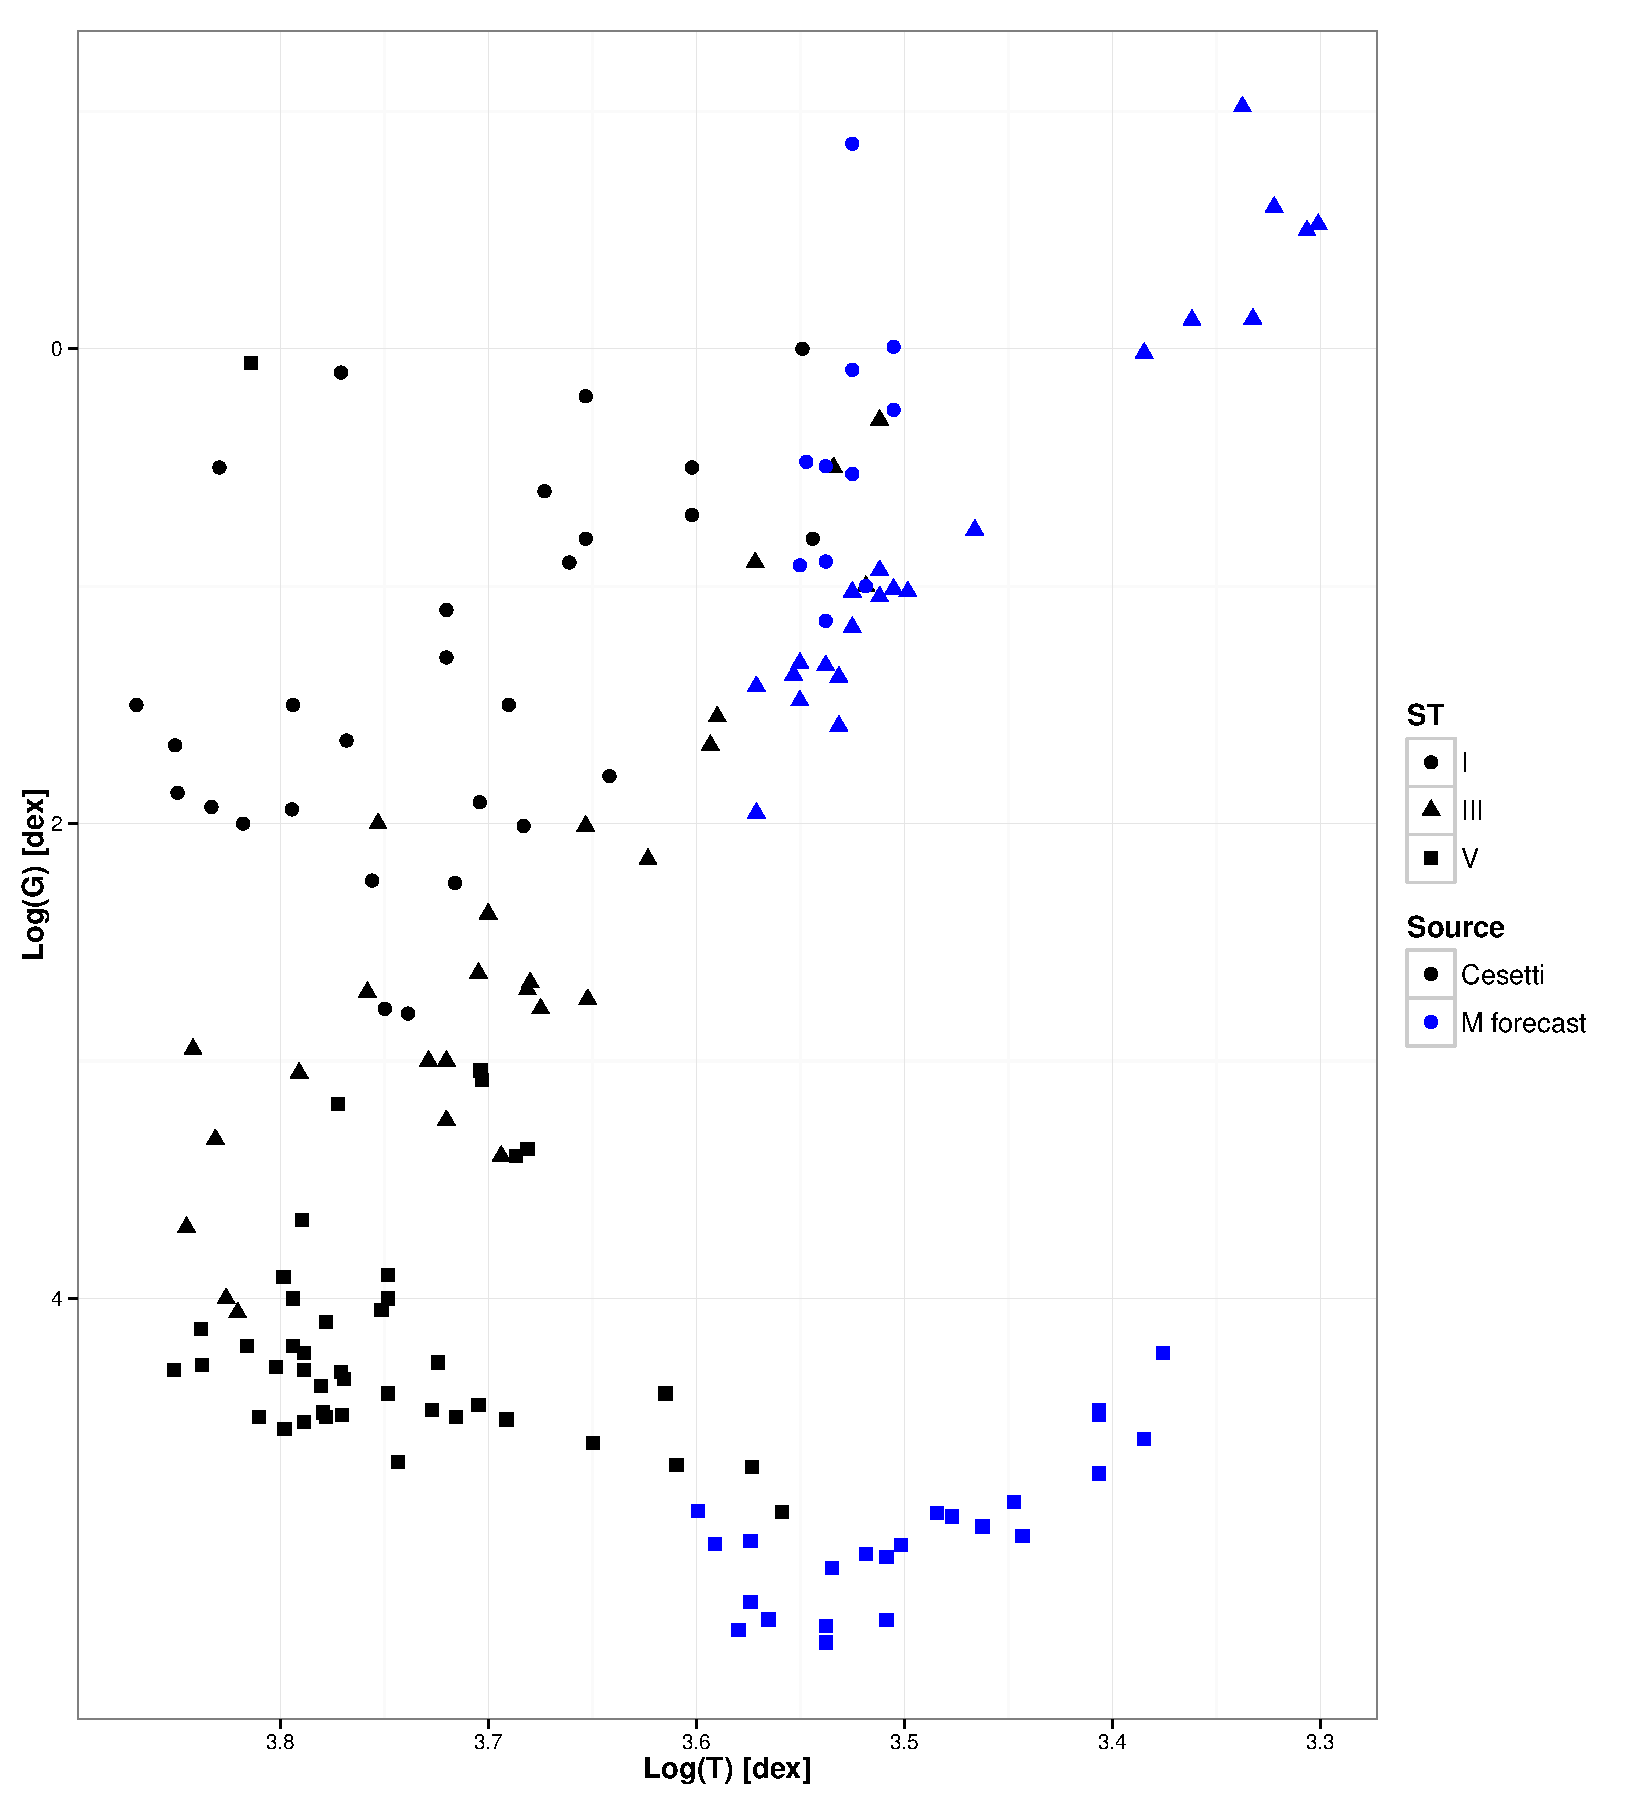
\includegraphics[width=12cm]{figs/irtf-logg-knn-oo.pdf}
 \caption{$\log(T_{eff})$--$\log(g)$ diagrams produced by the ???,
   ???, ???, and ??? models.}
 \label{fig:lt_lg_ga}
 \end{center}
\end{figure}

{\bf Is $chi^2$ much worse now for the weak parameter logg?}
%In this particular case, it is possible to see how 
%considering the global spectrum is positive for stronger 
%physical parameters like $T_{eff}$ but the approach
%reduces drastically its likelihood when other softer 
%parameters are involved.

\subsection{Metallicity models} 

Finally, the same machine learning models are trained to infer the
metallicity, again considering the effective temperature as an input
feature as in the $\log(g)$ regression
models. Table~\ref{tab:models_M_rmse} shows the cross-validation
results obtained for the same regression models considered in previous
Sections. Since only seven M-type stars in Table 3 of \cite{cesetti}
have metallicity estimates, the validation of our models with external
data is of little statistical significance. 
%
% Metalicidad teórica desde Cesseti para las IRTF
%
\ra{1.3}
\begin{table*}\centering
\begin{tabular}{@{}rrrcrrcrr@{}}\toprule
& \multicolumn{2}{c}{$SNR = 10$} & \phantom{ab}& \multicolumn{2}{c}{$SNR = 50$} &
\phantom{ab} & \multicolumn{2}{c}{$SNR = \infty$}\\
\cmidrule{2-3} \cmidrule{5-6} \cmidrule{8-9}
$Regression Models$ & $RMSE$ & $RMDSE$ && $RMSE$ & $RMDSE$     && $RMSE$       & $RMDSE$ \\ \midrule
$\chi^2$    & 0.76 & 0.22      && 0.36 & 0.18     && 0.36 & 0.18 \\
$PPR-ICA$   & 0.24 & \bf{0.13} && 0.31 & 0.22     && 0.43 & 0.27 \\
$GA-RF$     & 0.33 & 0.25      && 0.73 & 0.41     && 0.61 & 0.36 \\
$GA-GBM$    & 0.27 & 0.19      && 0.70 & 0.52     && 0.63 & 0.35 \\
$GA-SVR$    & 0.33 & 0.22      && 0.45 & 0.32     && 0.92 & 0.89 \\
$GA-NNET$   & 0.37 & 0.30      && 0.33 & 0.37     && 0.95 & 0.81 \\
$GA-KNN$    & 0.69 & 0.55      && 0.23 & \bf{0.15}&& 0.21 & \bf{0.15} \\ 
$GA-MARS$   & 0.36 & 0.16      && 0.49 & 0.41     && 0.83 & 0.85 \\
$GA-RR$     & 0.31 & 0.17      && 0.30 & 0.24     && 0.78 & 0.23 \\

\bottomrule
\end{tabular}
\caption {RMSE and RMDSE for the various regression models predicting
  metallicity [dex].}
\label{tab:models_M_rmse} 
% \end{center}
\end{table*}

{\bf Compare the 7 or 6 values available. Discuss.}  {\bf $\chi^2$ is
  the most popular method by far. We compare predictions of machine
  learning methods with minimum chi-squared. We first do histogram
  plots. Then, the same logTeff-logg plots as above but with
  metallicity coded in colour.}

% In Figure~\ref{fig:M_chi2_50_cesetti} and Figure~\ref{fig:M_GAM_1010_Cesetti} 
% relationships between metalicity predicted by global espectrum estimation 
% and GA feature based estimation against the real values
% provided by \cite{2013A&A...549A.129C} can be observed.

% \begin {figure}
%  \centering
%  \begin{subfigure}{.85\textwidth}
%   \centering
%   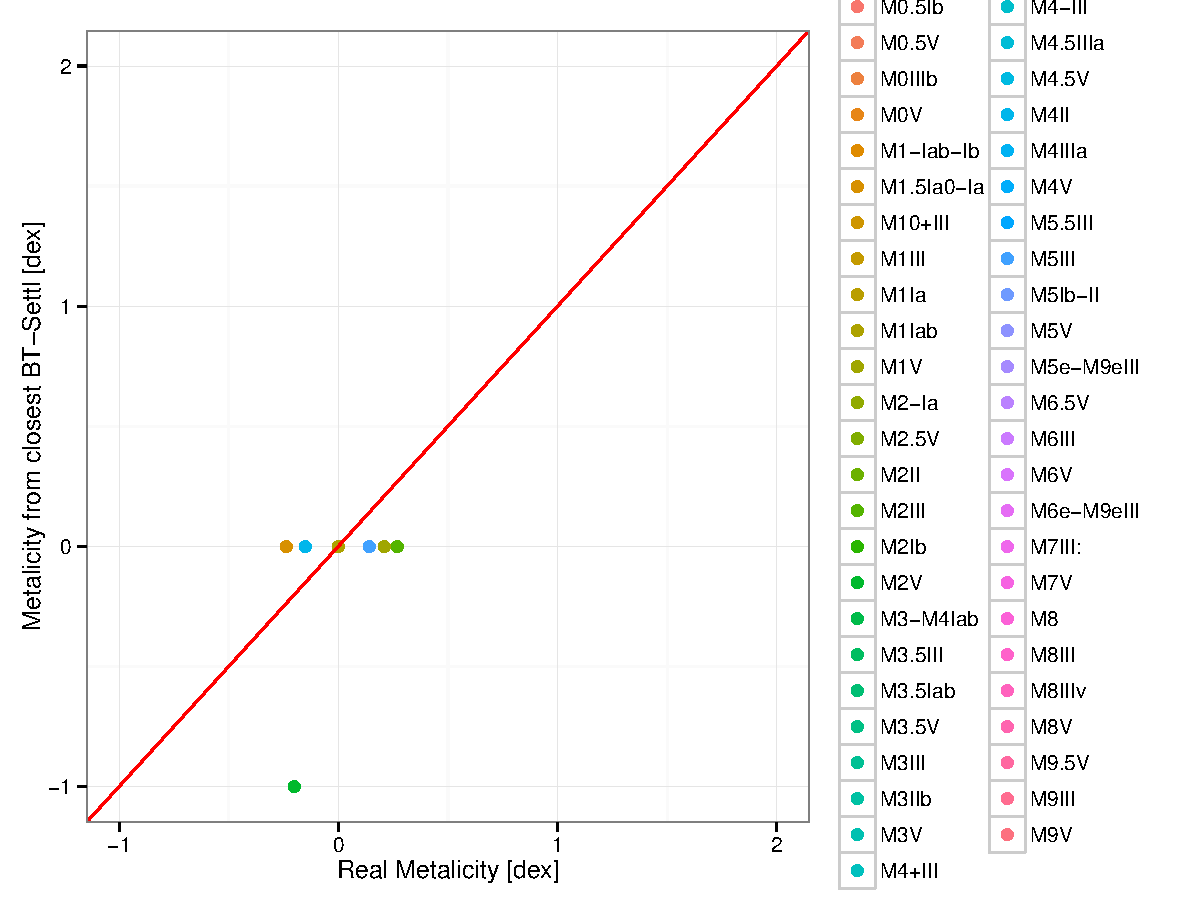
\includegraphics[width=12cm]{figs/M_Chi2_50_Cesetti.pdf}
%   \caption{Comparison between Metalicity estimations from Spectral Subtype 
%  in x axis and the closest BT\_Settl spectra by $\chi^2$ at SNR=$50$ on y-axis}
%  \label{M_chi2_50_cesetti}
%  \end{subfigure}
%   \begin{subfigure}{.85\textwidth}
%   \centering
%   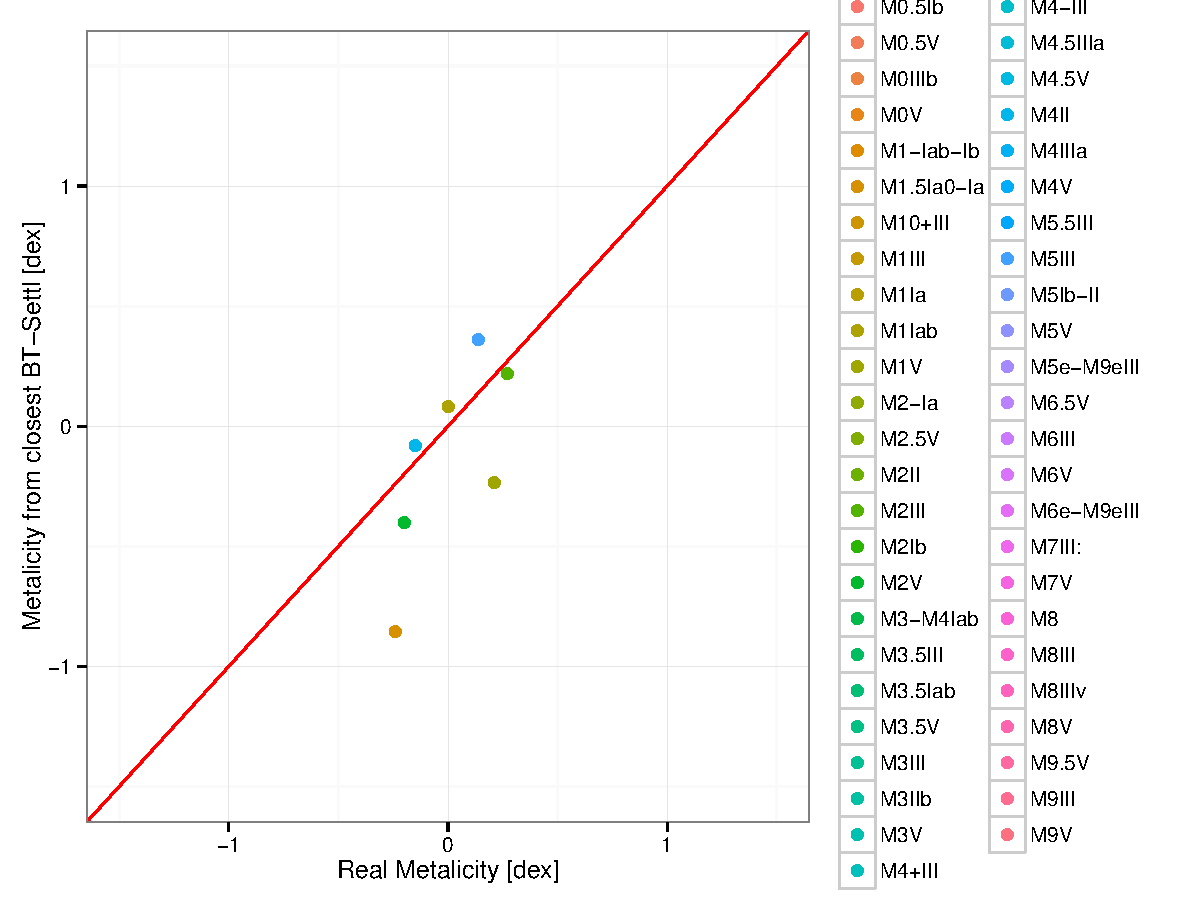
\includegraphics[width=12cm]{figs/M_GAM_1010_Cesetti.pdf}
%   \caption{Comparison between Metalicity estimations from Spectral Subtype 
%  in x axis and the Support Vector Machines for Ga based features trained with BT\_Settl 
%  at SNR=$\infty$ and features for forecasting at SNR=$\infty$ on y-axis}
%  \label{fig:M_GAM_1010_Cesetti}
%  \end{subfigure}
%  \label {fig:comp03}
%  \caption{Performance comparison between the $chi^2$ based selection 
%           and the band oriented features to forecast Log(g)}
% \end {figure}
%


\section{Physical parameters of the IPAC collection of spectra.}
%\input{ipac}
\subsection{Spectral bands selected}

As for the IRTF spectra, the spectral resolution of the BT-Settl
library was degraded to match the average resolution of IPAC spectra
in the Dwarf
Archives\footnote{http://spider.ipac.caltech.edu/staff/davy/ARCHIVE/index.shtml}. Then,
the spectra were trimmed to produce segments in the spectral range
common to all spectra of M stars in the archive, to avoid missing data
in the input variables. Finally, all spectra were divided by the total
integrated flux in this range in order to factor out the stellar
distance.

There is little hope {\it a priori} for reasonable accuracies with
regression models that predict the surface gravity and metallicity
from such wavelength-limited, low/intermediate resolution
spectra. Anyhow, we provide the results obtained applying the same
methodology as in Section \ref{sec:irtf} (and described in
Section \ref{sec:meth}) to show the limitations.

{\bf The application of the GA to the selection of features for the
prediction of effective temperature within the Dwarf Archives
wavelength range and resolution results in the features included in
Table~\ref{tab:ipac-teff-noisy}. Features are ordered by the fitness
value (according to the AIC criterion presented in Eq.~\ref{eq:AIC}),
and we only consider features that are present in at least 5 sets.}
%For the noisy spectra of SNR=10 and 50 we select
%the spectral features listed in Table~\ref{tab:ipac-teff-noisy}.

Table   %\ref{tab:ipac-logg-noiseless} and 
\ref{tab:ipac-logg-noisy}
shows the spectral features selected by the GA for noiseless BT-Settl
spectra and the same spectra with SNR=10 and 50, respectively.

Finally, the best features found by the GA for the estimation of the
metallicity are listed in 
% Table~\ref{tab:ipac-met-noiseless} for the
% noiseless BT-Settl spectra, and in 
Table~\ref{tab:ipac-met-noisy} for
signal-to-noise ratios equal to $\infty , 10 $ and $ 50 $.


\subsection{Regression models}

In the following, we will summarise the results obtained for the IPAC
data set. We deal with the different physical paramenters in separate
Sections. We start by reporting the cross validation Root Mean Square
Errors (RMSE) for the five-fold cross-validation strategy, and
subsequently discuss the accuracy of the predictions with respect to
literature values where available.

\subsection{Effective temperature models}

Table \ref{tab:model_IPAC_TSD} summarises the RMSE for the complete set of
models: the minimum $\chi^2$ estimate based on the full spectrum
($\chi^2$), the projection pursuit regression based on the ICA
components (PPR-ICA) and some models trained on the spectral
features proposed by the GA (GA-RF, 
GA-GBM, GA-SVR, GA-NNET, GA-MARS, GA-KPLS). For each model, we report
the RMSE obtained for several noise levels of the training sets. 
We use the following notation: RMSE represents the RMSE
obtained for a model trained and tested on BT Settl spectra. 
SNR=$\infty$ corresponds to noiseless spectra. 
The RMDSE means the root median square error, as a way to provide 
robust estimation against outliers.

Theoretical estimation about Temperature is carried out by Dr Sarro\textquoteright s 
relationship against subspectral type.

\newcommand{\ra}[1]{\renewcommand{\arraystretch}{#1}}
\begin{table*}\centering
\ra{1.3}
\begin{tabular}{@{}rrrcrrcrr@{}}\toprule
& \multicolumn{2}{c}{$SNR = 10$} & \phantom{ab}& \multicolumn{2}{c}{$SNR = 50$} &
\phantom{ab} & \multicolumn{2}{c}{$SNR = \infty$}\\
\cmidrule{2-3} \cmidrule{5-6} \cmidrule{8-9}
$Regression Models$ & $RMSE$ & $RMDSE$ && $RMSE$ & $RMDSE$ && $RMSE$ & $RMDSE$ \\ \midrule
$\chi^2 BTSettl$    &  147.48 & 79.02 && 121.40 & 55.78 && 126.03 & 57.26 \\
$ ICA+ ppr$         & 188.50 & 125.89 && 164.24 & 94.71 && 190.90 & 130.09 \\
$rf $               & 160.04 & 97.20 && 195.72 & 103.00 && 145.18 & 94.12 \\
$ gbm $             & 175.35 & 104.55 && 225.43 & 99.44 && 184.56 & 94.02 \\
$ svr $             & 203.11 & 112.06 && 284.93 & 106.29 && 367.65 & 153.64 \\
$ nnet $            & 220.97 & 83.91 && 313.43 & 111.41 && 394.81 & 202.17 \\
$ knn $             & 183.20 & 118.86 && 192.93 & 109.04 && 223.81 & 109.66  \\
$ mars+ bagging $   & 222.45 & 76.11 && 360.74 & 102.74 && 373.72 & 156.74 \\
$ kpls $            & 227.00 & 72.27 && 331.27 & 122.78 && 408.55 & 207.89 \\

\bottomrule
\end{tabular}
\caption {RMSE and RMDSE for the various regression models that predict $T_{eff}$ (K).} 
\label{tab:model_TSD} 
% \end{center}
\end{table*}


%

Most models show remarkably similar distributions of the
predictions when trained with different SNR levels. In the cases of
GA-MARS, GA-KNN, and GA-SVR this is the case even in the unrealistic
scenario of SNR=$\infty$.

In general, models tends to produce better behaved solutions (with
smaller biases and less scatter) for SNR=10. 

Major conclusion is that Temperature related features are distributed
throughout all the spectrum instead of being concetrated over specifc
bands. The reason for that is the $\chi^2$ estimator over the whole 
spectrum but the Independent Component Analysis based projections,
which behaves similarly by considering the whole spectrum.
In the same sense aproximations based on specific features performs
slightly worse that the whole spectrum, which confirms the spreaded 
features over the wavelength.

{\bf I should move this explanation to the beginning of the
section or to the methodology section.}


In Figures~\ref{fig:comp01}~\ref{fig:comp02} the relationship between Temperature
estimated from the GA technique proposed features and modeled with different 
technqiues and the $chi^2$ with SNR=50 against the 
estimations provided by Temperature estimated from 
the star\textquoteright spectral subtype can be seen.

\begin {figure}
 \centering
 \begin{subfigure}{.85\textwidth}
  \centering
  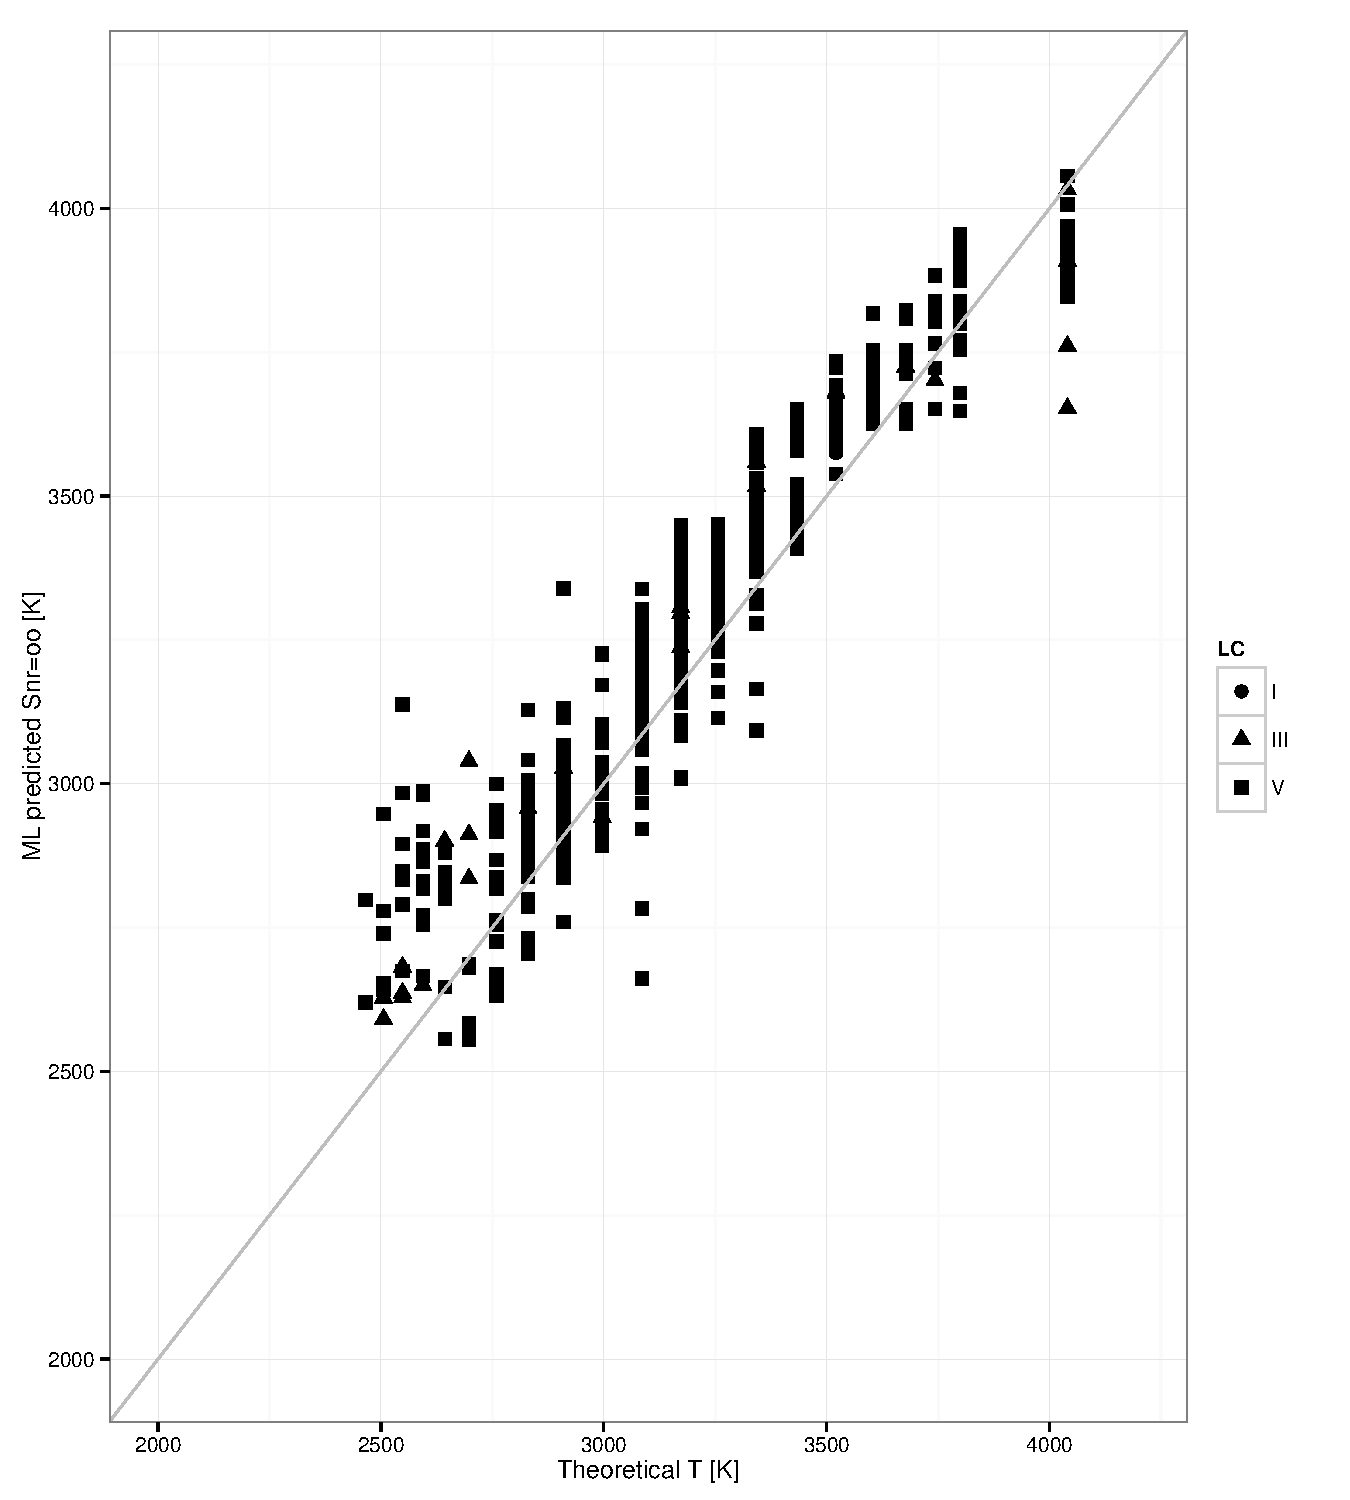
\includegraphics[width=11cm]{figs/ipac_T_ICAoo_LSB.pdf}
  \caption{Comparison between Temperature estimations from Theoretical Temperature 
  in x axis and the modeled ICA based estimation at SNR=$\infty$ on y-axis}
 \label{fig:ipac_icaoo_lsb}
 \end{subfigure}
  \begin{subfigure}{.85\textwidth}
  \centering
  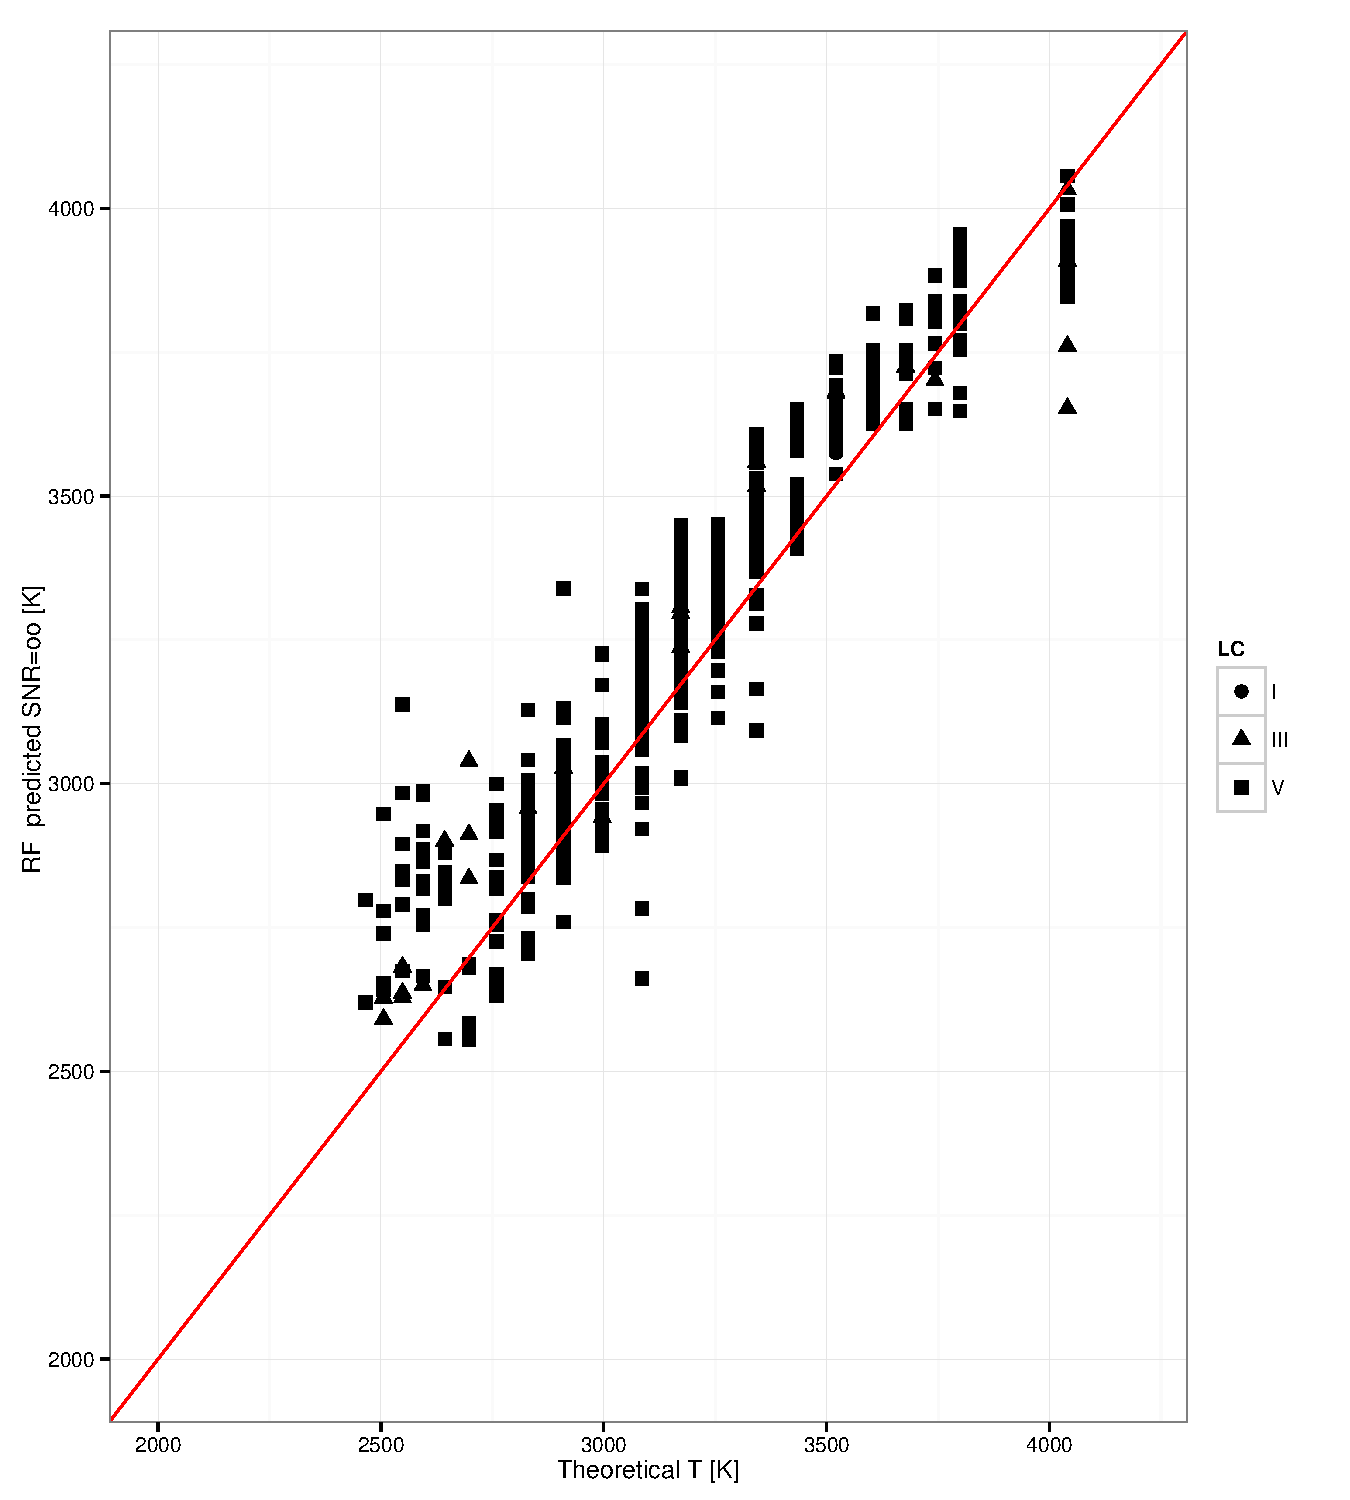
\includegraphics[width=11cm]{figs/ipac_T_RFoo_LSB.pdf}
  \caption{Comparison between Temperature estimations from Theoretical Temperature 
  in x axis and the featured based Random Forest modeled at SNR=$\infty$ on y-axis}
 \label{fig:ipac_rfoo_lsb}
 \end{subfigure}
  \begin{subfigure}{.85\textwidth}
  \centering
  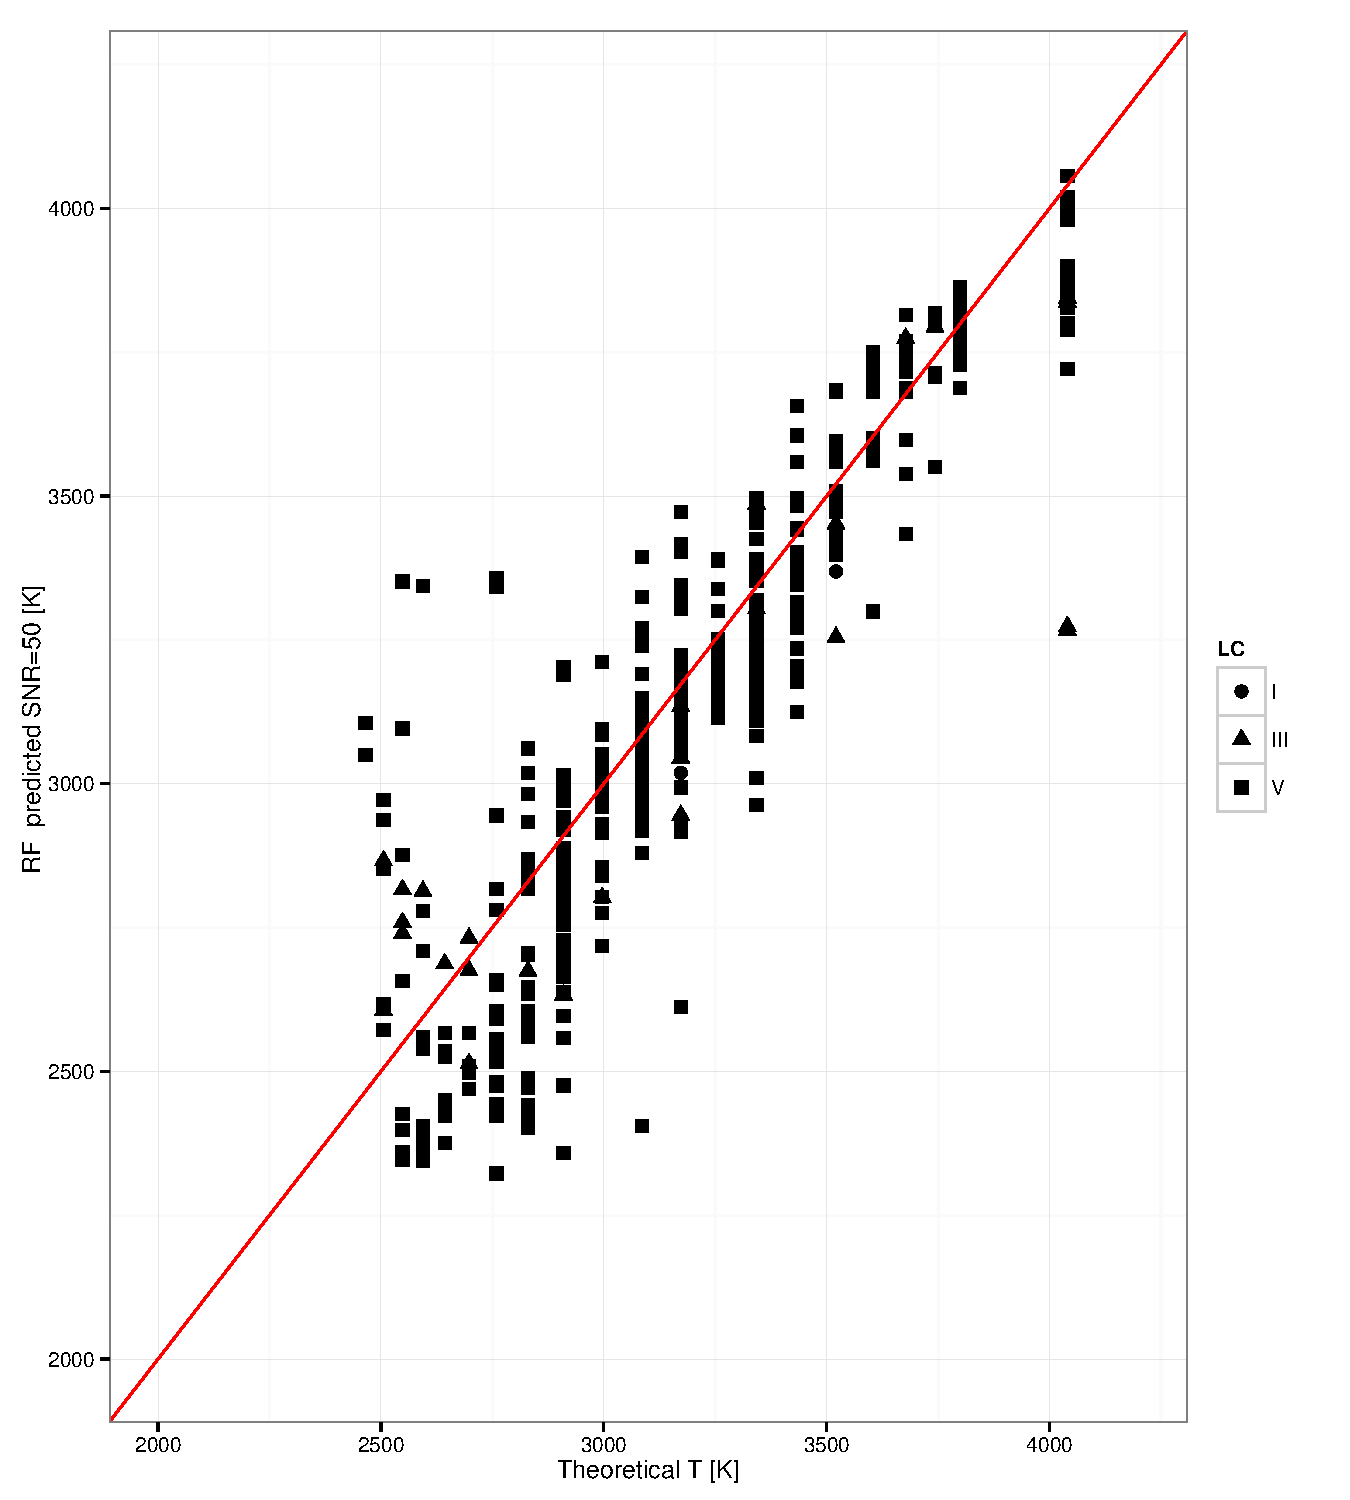
\includegraphics[width=11cm]{figs/ipac_T_RF50_LSB.pdf}
  \caption{Comparison between Temperature estimations from Theoretical Temperature 
  in x axis and the featured based Random Forest modeled at SNR=$\50$ on y-axis}
 \label{fig:ipac_rf50_lsb}
 \end{subfigure}
 \label {fig:comp01}
 \caption{Performance comparison between the different strategies for Teperature prediction}
\end {figure}
 
 
We can produce a comparison with the features provided by Cesetti, within the I band range
making sense for the IPAC spectra (see Table \ref{tab:tab_CS_T}).
\begin{table}
\begin{center}
\begin{tabular}{rrrr}
  \hline
  $\lambda_1$ & $\lambda_2$ & $\lambda_{cont;1}$ & $\lambda_{cont;2} $ \\ 
  \hline
8461 & 8474 & 8474 & 8484 \\
8484 & 8513 & 8474 & 8484 \\
8522 &  8562 & 8474 & 8484 \\
8577 & 8619 & 8563 & 8577 \\
8642 & 8682 & 8619 & 8642 \\
8730 & 8772 & 8700 & 8725 \\
8802 & 8811 & 8776 & 8792 \\
8850 & 8890 & 8815 & 8850 \\
9000 & 9030 & 8983 & 8998 \\
9080  & 9100 & 9040 & 9050 \\

\hline
\end{tabular}
\caption {Features selected by following suggestions from Cesetti et al, table 1. } 
\label{tab:tab_CS_T}
\end{center}
\end{table}

We have built nonlinear models with the same method we did for the features suggested 
by the GA techniques, learning from BT-Settl as a whole and predicting over the IPAC set
(see \ref{tab:tab_CS_Model}).

\begin{tabular}{@{}rrrcrrcrr@{}}\toprule
& \multicolumn{2}{c}{$SNR = 10$} & \phantom{ab}& \multicolumn{2}{c}{$SNR = 50$} &
\phantom{ab} & \multicolumn{2}{c}{$SNR = \infty$}\\
\cmidrule{2-3} \cmidrule{5-6} \cmidrule{8-9}
$Regression Models$ & $RMSE$ & $RMDSE$ && $RMSE$ & $RMDSE$     && $RMSE$       & $RMDSE$ \\ \midrule
$rf $               & 202.86 & 139.65 && 243.13 & 120.82 && 305.72 & 171.58  \\
$gbm $              & 187.70 & 120.04 && 160.76 & 138.07 && 336.78 & 222.11  \\
$ svr $             & 196.85 & 134.66 && 379.36 & 193.56 && 840.30 & 688.47  \\
$ nnet $            & 206.89 & 135.18 && 513.71 & 295.86 && 719.28 & 489.00  \\
$ mars+ bagging $   & 252.03 & 123.70 && 789.30 & 186.29 && 3464.16 & 784.14  \\
$knn  $             & 235.29 & 158.22 && 246.17 & 136.75 && 313.88 & 175.02  \\
$ kpls $            & 250.14 & 200.68 && 741.48 & 361.14 && 2246.74 & 1424.20  \\
$Rule Regression $  & 210.81 & 128.07 && 400.04 & 238.60 && 828.00 & 774.26  \\

\hline
\end{tabular}
\caption {Regression models performance based on Cesetti features} 
\label{tab:tab_CS_Model}
\end{center}
\end{table}



\subsection{Surface gravity models}

The same approach can become useful to produce $log(G)$ estimations. 
Here comparisons can only be possible between GA based features, the 
global spectra based approach with $\chi^2$ distance
to be minimized and those stars with gravity was 
estimated in  \cite{2013A&A...549A.129C}.

The only difference with the methodology presented above is because
Temperature has been considered a fixed feature in the estimation of 
Gravity.

In Table~\ref{tab:models_G_rmse} 
we can see the analysis of performance between
the $\chi^2$ identificacion and the one based on features from the spectrum
depending on several classes of features. The checks were carried out against 
$Log(g)$ from Rojas-Ayala.

%
% Gravedad teórica desde Cesseti para las IRTF
%
\ra{1.3}
\begin{table*}\centering
\begin{tabular}{@{}rrrcrrcrr@{}}\toprule
& \multicolumn{2}{c}{$SNR = 10$} & \phantom{ab}& \multicolumn{2}{c}{$SNR = 50$} &
\phantom{ab} & \multicolumn{2}{c}{$SNR = \infty$}\\
\cmidrule{2-3} \cmidrule{5-6} \cmidrule{8-9}
$Regression Models$ & $RMSE$ & $RMDSE$ && $RMSE$ & $RMDSE$     && $RMSE$       & $RMDSE$ \\ \midrule
$\chi^2 BTSettl$    &  2.20     & 1.62  && 2.19 & 1.49 && 2.24  & 1.56 \\
$ ICA+ ppr$         & \bf{2.14} & 1.78  && \bf{1.82} & 1.71 && 4.31  & 4.18 \\
$rf $               & \bf{1.35} & \bf{0.97} && \bf{1.62} & \bf{1.12} && \bf{1.41} & \bf{0.93} \\
$gbm $              & \bf{1.59} & \bf{1.15} && \bf{1.69} & \bf{1.37} && \bf{1.66} & \bf{1.17} \\
$ svr $             & \bf{1.98} & 1.81  && \bf{2.13} & 1.88  && 2.28 & 1.58 \\
$ nnet $            & \bf{2.03} & 1.78  && 2.25 & 1.95 && 3.22 & 2.78 \\
$ mars+ bagging $   & \bf{1.85} & \bf{1.55} && \bf{2.03} & 1.73 && \bf{2.03}  & \bf{1.50} \\
$knn  $             & \bf{2.05} & \bf{1.54} && 2.18 &  1.73  &&  \bf{1.71} & \bf{1.19} \\
$ kpls $            & \bf{1.85} & \bf{1.44} && \bf{2.01} & 1.72 && 2.75 & 2.31 \\
$Rule Regression $  & \bf{2.01} & 1.76 && \bf{2.09} & 1.80 && 3.73 &  3.22 \\

\bottomrule
\end{tabular}
\caption {RMSE and RMDSE for the various regression models predicting $Log(G)$ [dex].} 
\label{tab:models_G_rmse} 
% \end{center}
\end{table*}


It is possible to present relationships between $log(g)$ and $log(T)$
as a matter of congruence analysis between predictions. In the Figure~\ref{fig:lt_lg_ga}
such relationship is presented for models based on artificial intelligence selected features.

\begin{figure}
 \begin{center}
 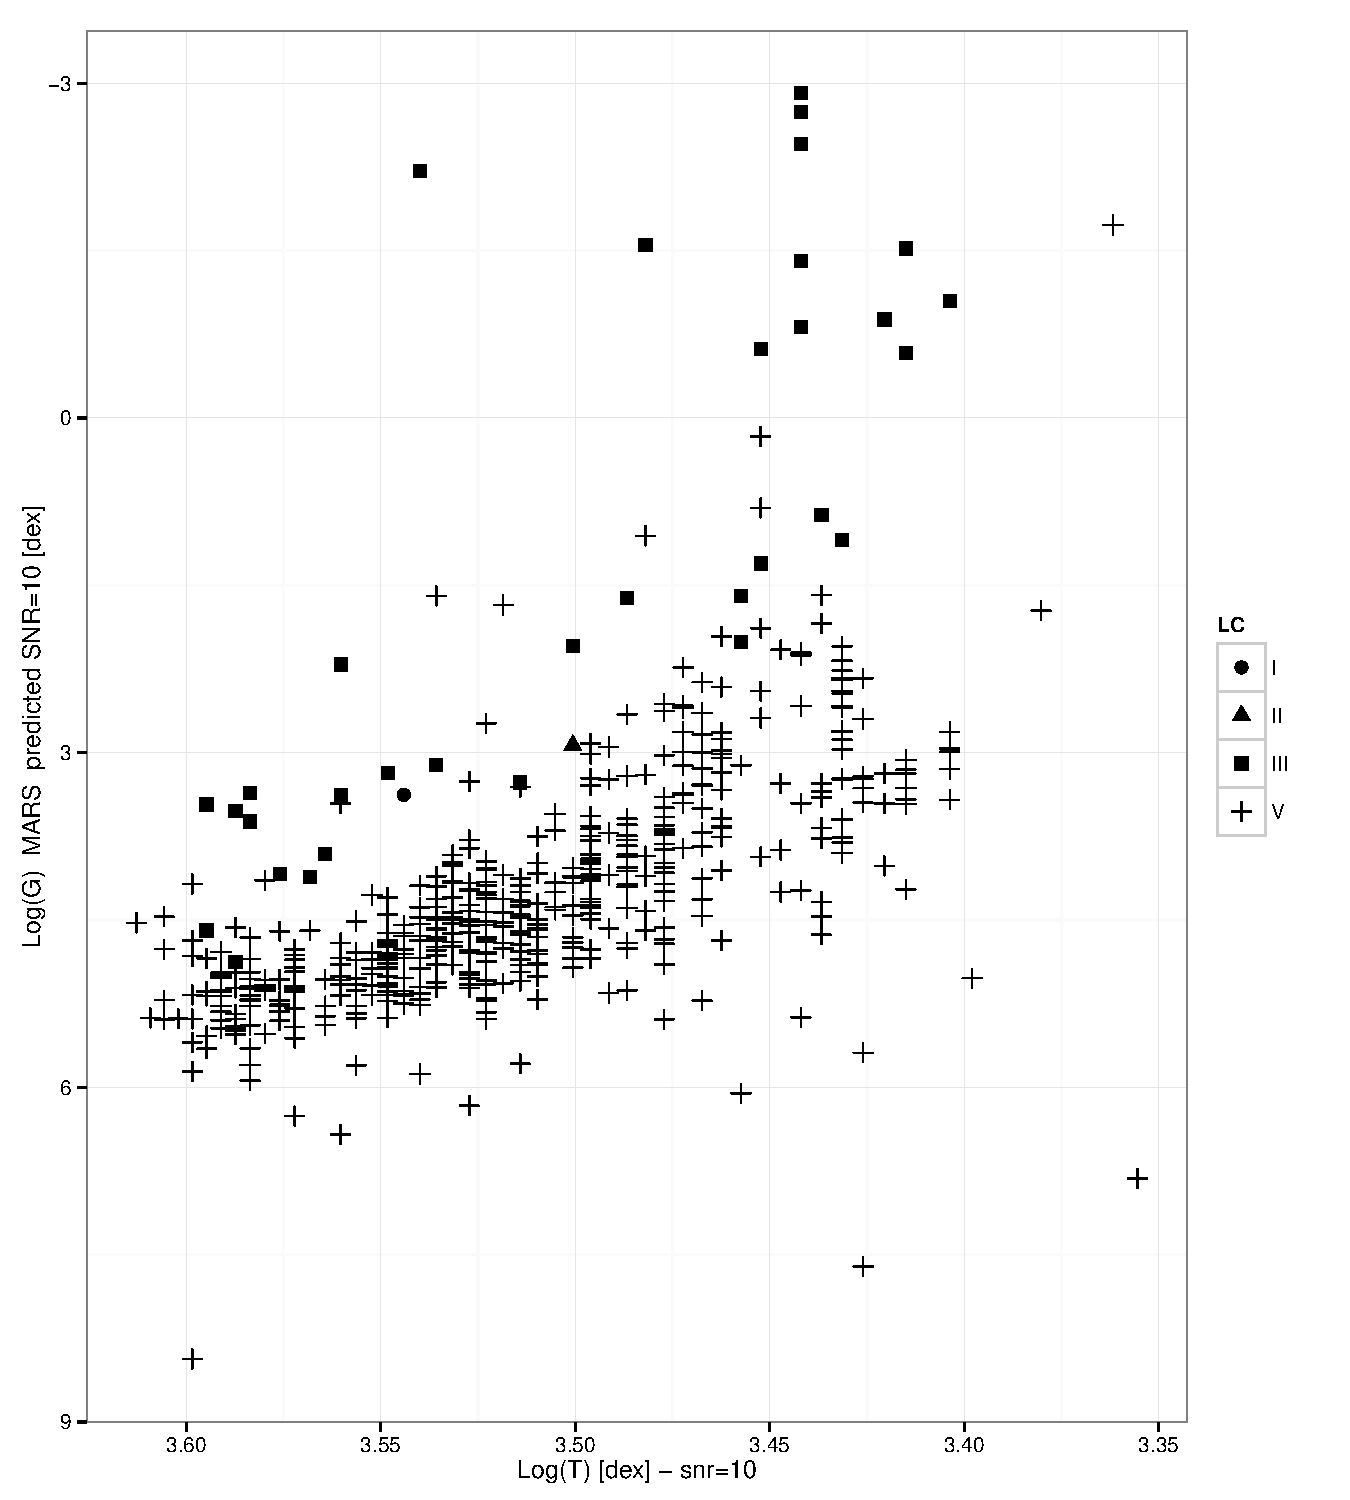
\includegraphics[width=12cm]{figs/ipac_LG_T_Mars_10.pdf}
 \caption{Relationship between $log(T) $ in the x axis 
 and $log(g)$ in the y axis for MARS model based on the GA provided bandpass features with SNR=$\10$}
 \label{fig:lt_lg_ga}
 \end{center}
\end{figure}

We can plot relationships between $log(g)$ and $log(T)$
as a matter of congruence analysis between predictions. In the Figure~\ref{fig:lt_lg_pls}
such relationship is presented.

\begin{figure}
 \begin{center}
 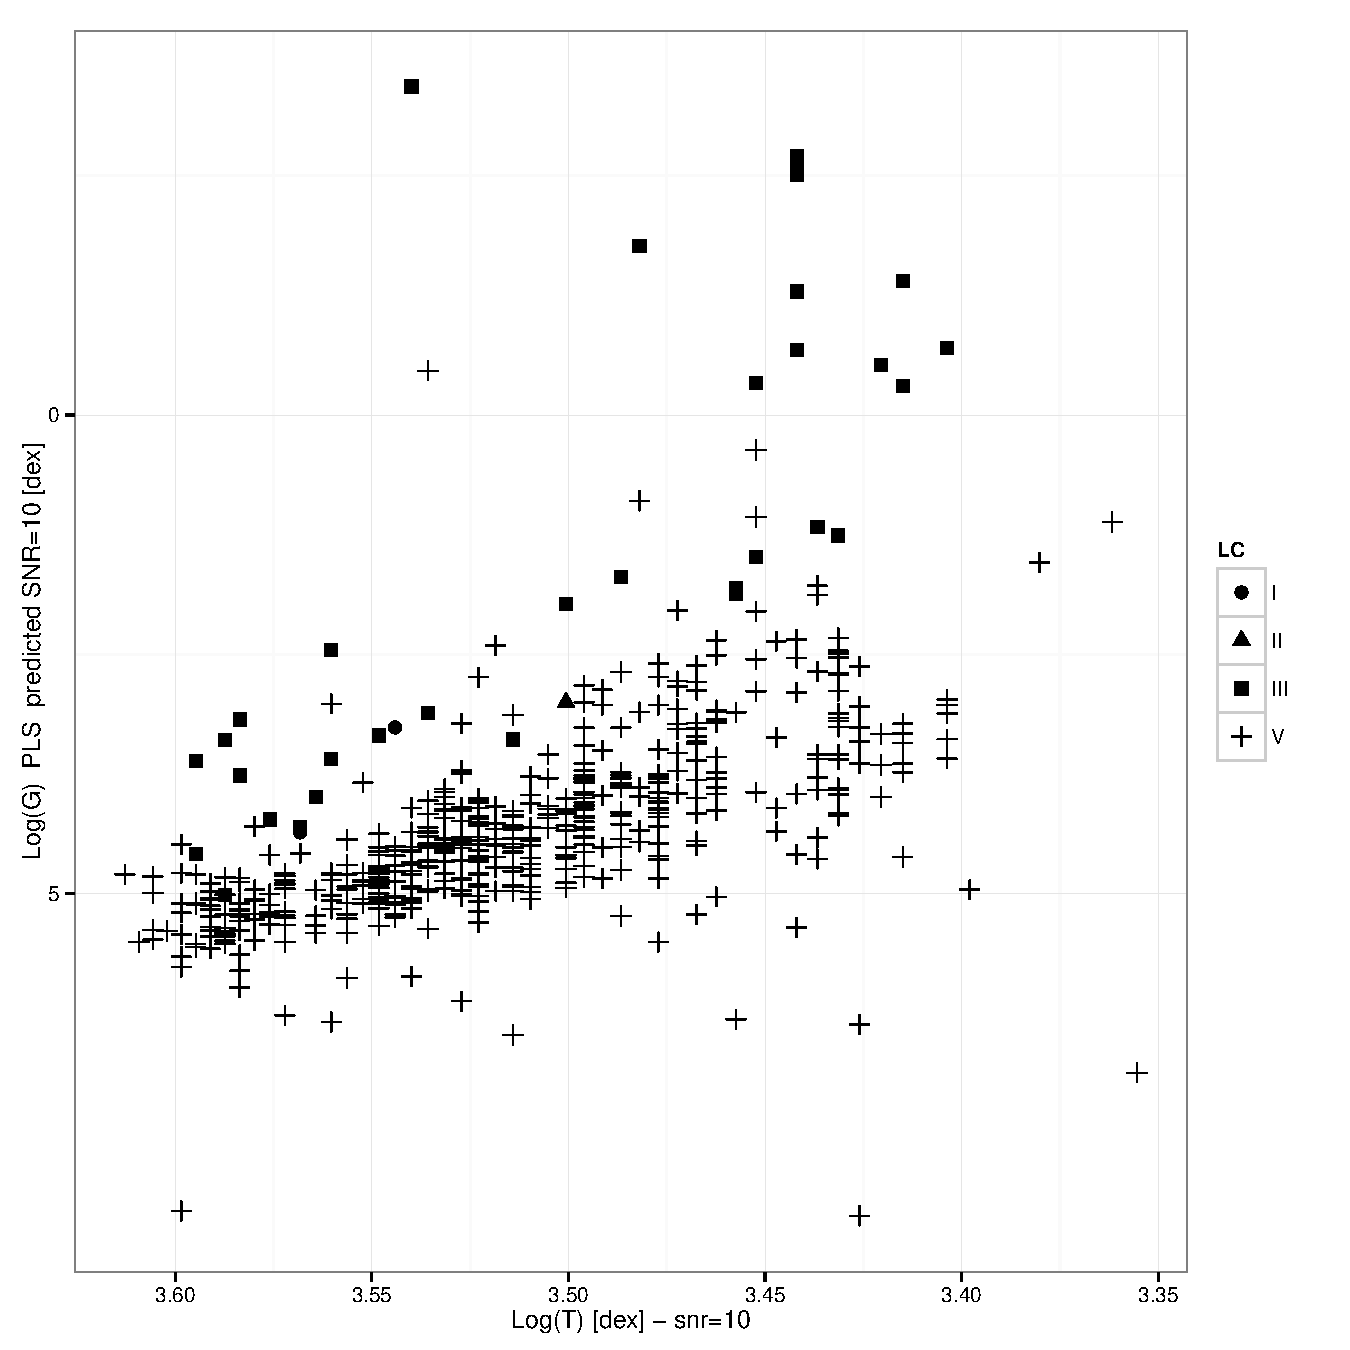
\includegraphics[width=12cm]{figs/ipac_LG_T_PLS_10.pdf}
 \caption{Relationship between $log(T) $ in the x axis 
 and $log(g)$ in the y axis for Partial Least Square model based on the GA provided bandpass features with SNR=$\10$}
 \label{fig:lt_lg_pls}
 \end{center}
\end{figure}

The relationship between the GA predicted Temperature and the one measured by Rojas-Ayala can be 
found in the Figure~\ref{fig:ipac_lt_lt}
\begin{figure}
 \begin{center}
 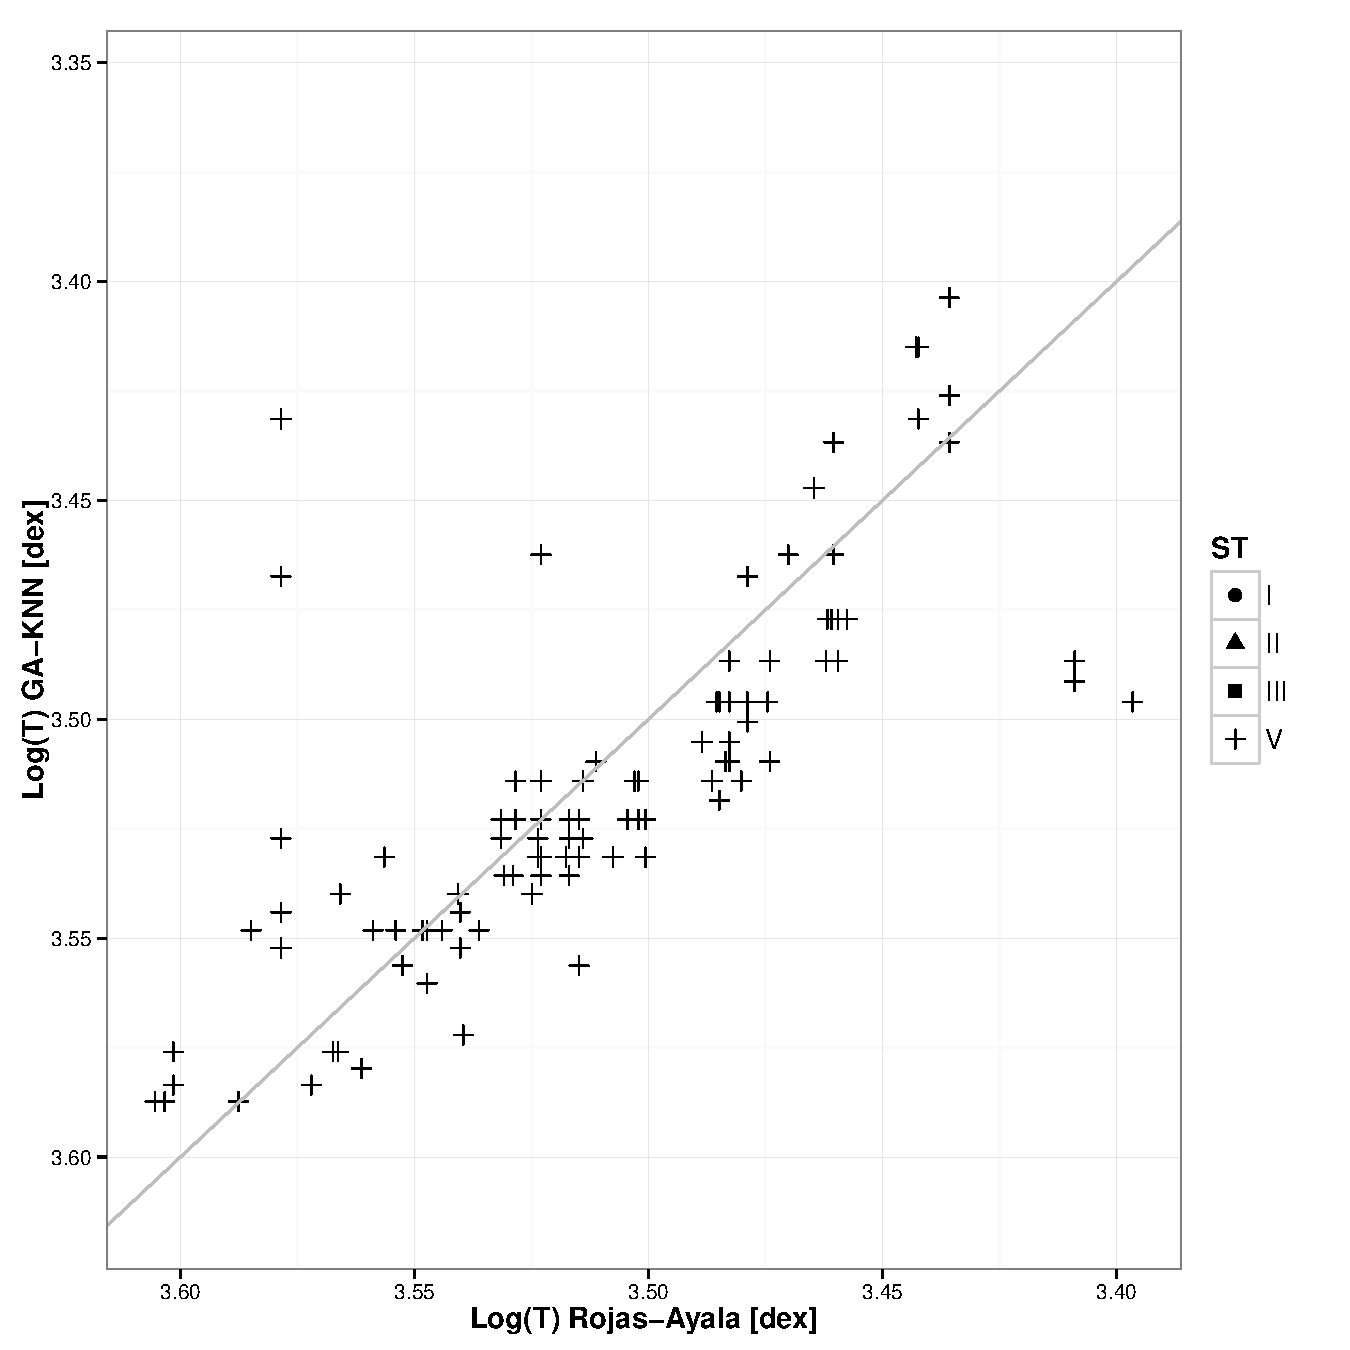
\includegraphics[width=12cm]{figs/ipac_LG_Trojas_Tknn_10.pdf}
 \caption{Relationship between $log(T) from Rojas-Ayala $ in the x axis 
 and $log(T)$ as predicted by KNN with SNR=$\10$}
 \label{fig:ipac_lt_lt}
 \end{center}
\end{figure}

\subsection{Metallicity models} 

Finally, the same analysis is performed for the Metalicty parameter, 
again by considering Temperature as a fixed feature.
In Table~\ref{tab:models_M_rmse} 
we can see the analysis of performance of different classes of
models and cosidering a variety in features. The checks were carried out against 
$Met$ from Neves III.

%
% Metalicidad teórica desde NevesIII para IPAC
%
\ra{1.3}
\begin{table*}\centering
\begin{tabular}{@{}rrrcrrcrr@{}}\toprule
& \multicolumn{2}{c}{$SNR = 10$} & \phantom{ab}& \multicolumn{2}{c}{$SNR = 50$} &
\phantom{ab} & \multicolumn{2}{c}{$SNR = \infty$}\\
\cmidrule{2-3} \cmidrule{5-6} \cmidrule{8-9}
$Regression Models$ & $RMSE$ & $RMDSE$ && $RMSE$ & $RMDSE$     && $RMSE$       & $RMDSE$ \\ \midrule
$\chi^2 BTSettl$    &  0.55    & 0.27   && 0.51 & 0.29 && 0.43  & 0.29 \\
$ ICA+ ppr$         & \bf{0.48} & 0.27 && 0.70  & 0.39 && 0.85  & 0.71 \\
$rf $               & 0.55 & 0.38    && 0.71  & 0.61   && \bf{0.23}  & \bf{0.16} \\
$gbm $              & 0.64 & 0.43 && 0.87  & 0.84  && \bf{0.31}  & \bf{0.23} \\
$ svr $             & \bf{0.46} & \bf{0.26}   && 0.57 & 0.44  && 3.38  & 2.33 \\
$ nnet $            & \bf{0.52} & 0.45      && 0.66 & 0.54  && 2.03  & 1.88 \\
$ knn $             & \bf{0.37}  & 0.28   && 0.99  & 0.78 && 0.56 & 0.32 \\ 
$ mars+ bagging $   & 0.71  & 0.47 && 0.80   & 0.69   && 1.15    & 0.68 \\
$ pls $             & 0.67  & 0.61  && 0.63  & 0.55 && 1.17 & 1.02 \\ 
$Rule Regression $  & \bf{0.47} & 0.29 && 0.50 & 0.36  && 1.18 &  1.18 \\

\bottomrule
\end{tabular}
\caption {RMSE and RMDSE for the various regression models predicting $Met$ [dex].} 
\label{tab:models_M_rmse} 
% \end{center}
\end{table*}



The relationship between the GA predicted Temperature and the one measured by Rojas-Ayala can be 
found in the Figure~\ref{fig:ipac_mt}
\begin{figure}
 \begin{center}
 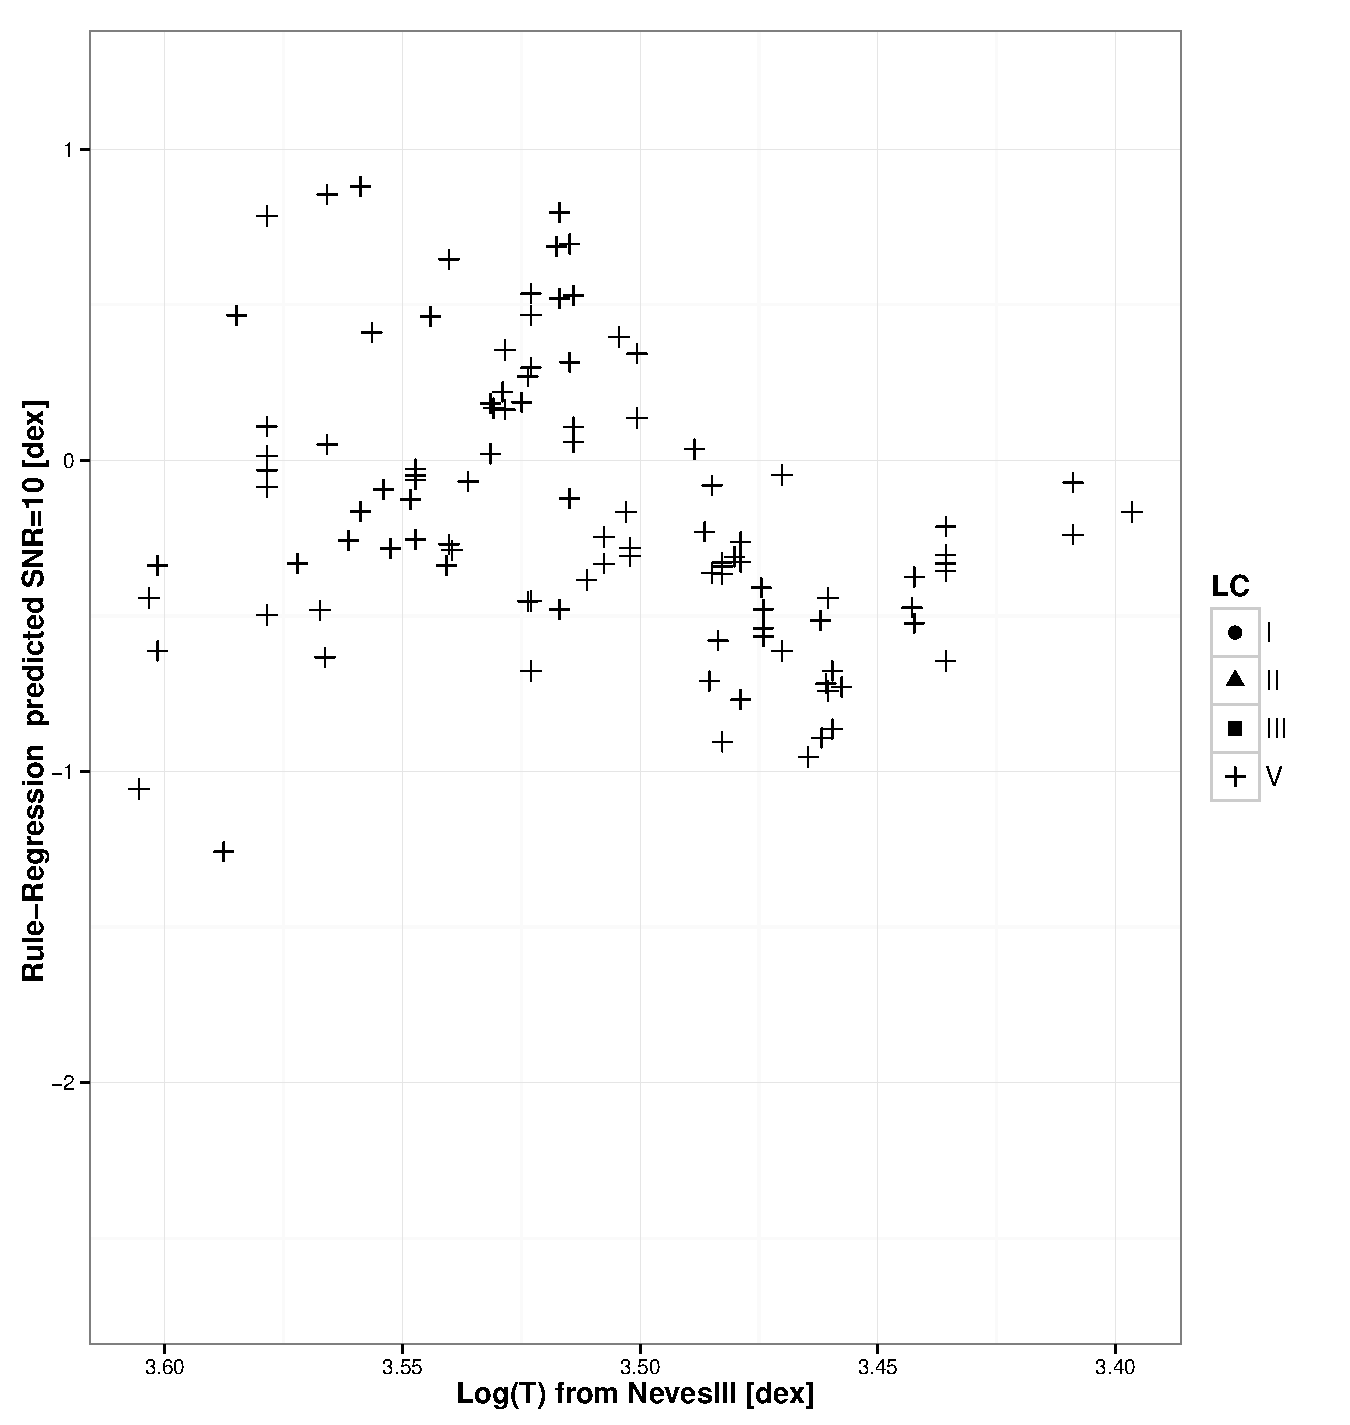
\includegraphics[width=12cm]{figs/ipac_Met_10_NevesIII.pdf}
 \caption{Relationship between $ T from NevesIII $ in the x axis 
 and $ Met $ as predicted by Regression Rules with SNR=$\10$}
 \label{fig:ipac_mt}
 \end{center}
\end{figure}


% In Figure~\ref{fig:M_chi2_50_cesetti} and Figure~\ref{fig:M_GAM_1010_Cesetti} 
% relationships between metalicity predicted by global espectrum estimation 
% and GA feature based estimation against the real values
% provided by \cite{2013A&A...549A.129C} can be observed.

% \begin {figure}
%  \centering
%  \begin{subfigure}{.85\textwidth}
%   \centering
%   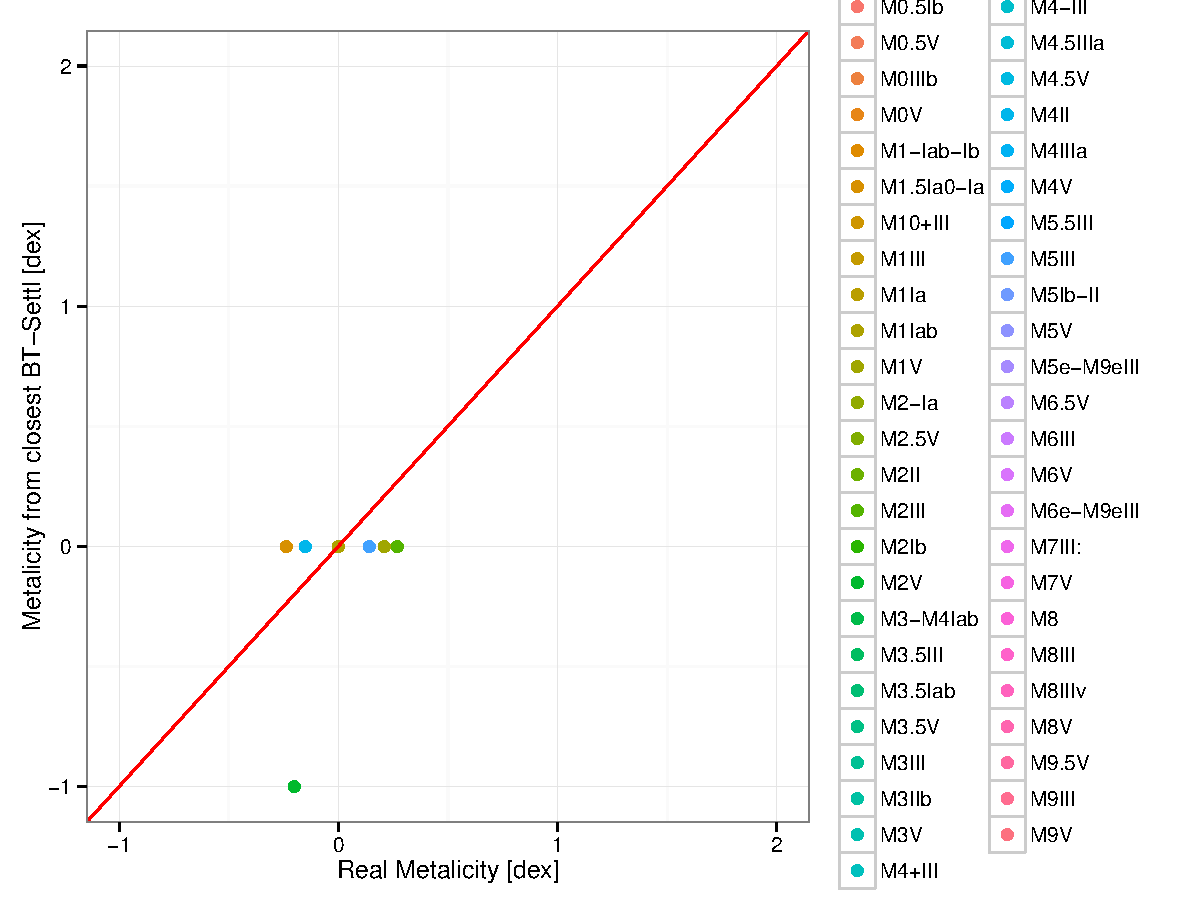
\includegraphics[width=12cm]{figs/M_Chi2_50_Cesetti.pdf}
%   \caption{Comparison between Metalicity estimations from Spectral Subtype 
%  in x axis and the closest BT\_Settl spectra by $\chi^2$ at SNR=$50$ on y-axis}
%  \label{M_chi2_50_cesetti}
%  \end{subfigure}
%   \begin{subfigure}{.85\textwidth}
%   \centering
%   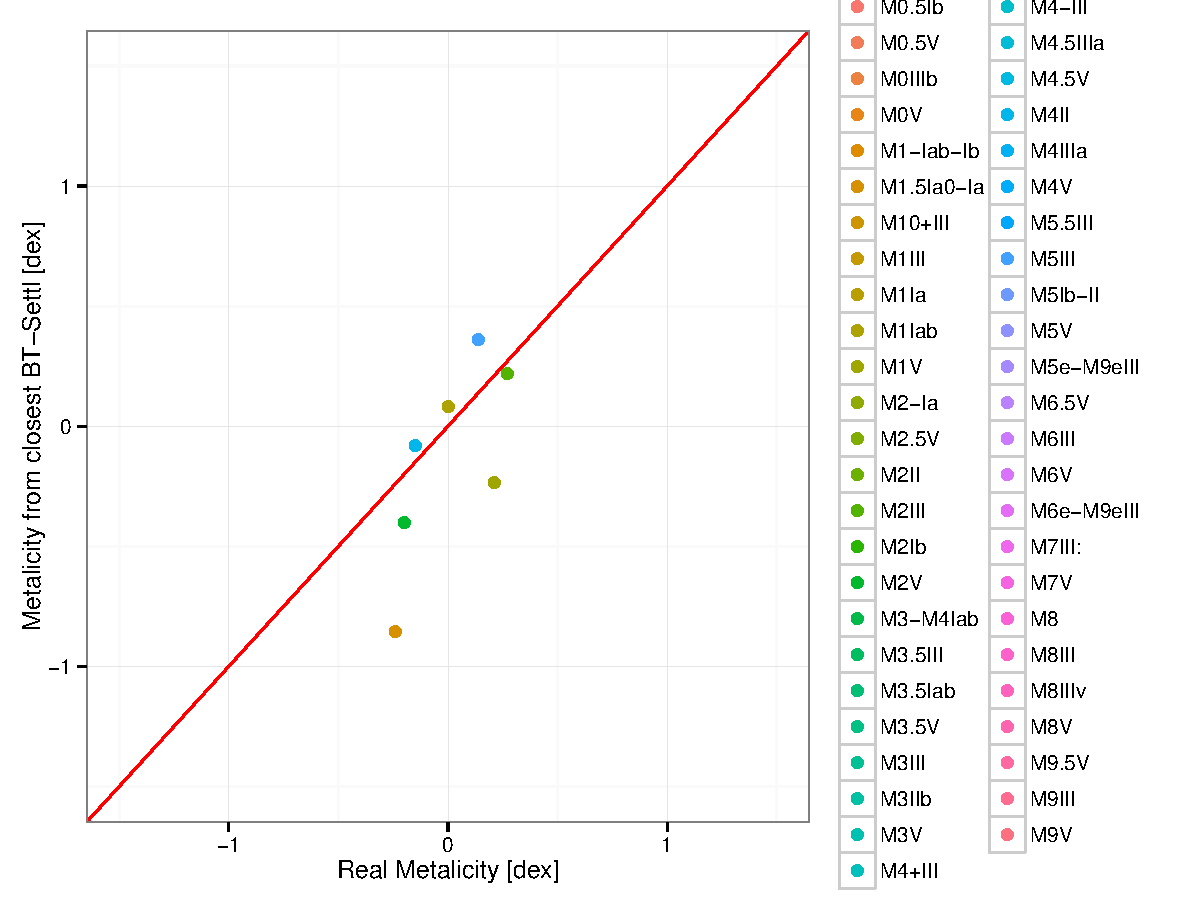
\includegraphics[width=12cm]{figs/M_GAM_1010_Cesetti.pdf}
%   \caption{Comparison between Metalicity estimations from Spectral Subtype 
%  in x axis and the Support Vector Machines for Ga based features trained with BT\_Settl 
%  at SNR=$\infty$ and features for forecasting at SNR=$\infty$ on y-axis}
%  \label{fig:M_GAM_1010_Cesetti}
%  \end{subfigure}
%  \label {fig:comp03}
%  \caption{Performance comparison between the $chi^2$ based selection 
%           and the band oriented features to forecast Log(g)}
% \end {figure}
%
   
   

% De nuevo, el análisis y discusión, función de lo que queramos dejar



\section{Conclusions}

\begin{acknowledgements}
This research has benefitted from the M, L, T, and Y dwarf compendium housed at DwarfArchives.org.
The authors also thanks to the Spanish Ministery for Economy and Innovation because of the 
support obtained through the project with ID: AyA2011-24052. IRTF library provided by the 
University of Hawaii under Cooperative Agreement no. NNX-08AE38A with the National 
Aeronautics and Space Administration, Science Mission Directorate, Planetary Astronomy Program.
\end{acknowledgements}

%-------------------------------------------------------------------

\bibliography{references_m}{}
\bibliographystyle{bibtex/aa}

\end{document}
